\documentclass[12pt]{book}


\usepackage{exercises}
\RequirePackage{lineno}
\usepackage{graphicx}
\usepackage{amsmath}
\usepackage[a4paper, total={6.3in, 8.5in}]{geometry}
\usepackage[super]{natbib}


%\usepackage{siunitx}
%\usepackage[version=3]{mhchem}
%\renewcommand*{\thefootnote}{\fnsymbol{footnote}}
%\graphicspath{ {../Figures/} }
\linespread{1}

\usepackage{geometry}
 \geometry{
 a4paper,
 left=20mm,
 right=20mm,
 top=25mm,
 bottom=20mm,
 }

% Makes nice font:
\renewcommand{\familydefault}{\sfdefault}

\newcommand{\DocTitle}{Climate Dynamics Course Notes}

\usepackage{fancyhdr}
\pagestyle{fancy}
\fancyhf{}
\rhead{Mauritsen}
\chead{}
\lhead{\DocTitle}
\cfoot{}
\cfoot{}

% Remove to get numbers:
%\bibliographystyle{plainnat}
%\bibpunct{(}{)}{;}{a}{}{,}


\newcommand{\beginsupplement}{%
        \setcounter{table}{0}
        \renewcommand{\thetable}{S\arabic{table}}%
        \setcounter{figure}{0}
        \renewcommand{\thefigure}{S\arabic{figure}}%
     }

%
%\begin{document}
%
%
%\begin{center}
%\noindent
%{\LARGE 
%\DocTitle
%} \\
%\vspace{0.5 cm}
%
%\noindent
%{\bf Thorsten  Mauritsen$^{1*}$}\\
%\today \\
%\end{center}
%
%\noindent
%$^1$ Max Planck Institute for Meteorology, Hamburg, Germany \\
%%$^2$ University of Colorado, Boulder, USA \\
%%$^3$ NOAA Earth System Research Lab, Physical Sciences Division, Boulder, USA \\
%\\
%$^*$ Corresponding author: Thorsten Mauritsen, Max Planck Institute for Meteorology, Bundesstrasse 53, 20146 Hamburg, Germany, e-mail: thorsten.mauritsen@mpimet.mpg.de\\
%
%%\linenumbersK
%%\linenumbers
%%\modulolinenumbers[2]


\title{\DocTitle}
\author{Thorsten Mauritsen}
\date{\today}
 
\begin{document}
 
\maketitle
\tableofcontents



\frontmatter
\cfoot{Page \thepage}
\chapter{Preface}
Let us take a look at a planet from space -- and -- imagine we let time pass relatively quickly. From this perspective we can observe a system in approximate stationarity; something which we usually call equilibrium. This is not to be mistaken for a strict thermodynamical equilibrium, wherein, as you may have learnt in other courses, the system is characterised by a single well-defined temperature, but rather an approximate equilibrium between radiative energy received from the star around which our planet of interest is circulating (provided it does have a star), and the thermal energy that the planet is radiating to space. How does the planet come into equilibrium, and is there only one equilibrium? How does the equilibrium change if the star changes it's irradiance, or the planets orbit is altered? How does the equilibrium of the planet depend on properties of the planet? To begin to answer these questions we will have to dig into the processes that determine the energy balance, but the starting point will be our somewhat abstract perspective from space and time.

Usually we think of the climate as something that is static, we think of averages in time -- traditionally taken to be 30 years; a rather arbitrary choice as it turns out. So why discuss the dynamics of something that is static? The climate is varying on timescales as short as we choose to define them up to those of the existence of the planet. These variations were either due to external factors, such as the sun, or  the composition of the atmosphere changing due to biogeochemical processes, or internal variability. Much of this can be described by simple dynamical equations, as the dynamics of climate. A related and interesting field describes the dynamics of the atmosphere and ocean circulations and their biogeochemical cycles. 

\vspace{1.0 cm}
\noindent
{\bf \LARGE Scope of the course}
\\
\\
\noindent In the Climate Dynamics course I hope to bring you close to the forefront of current knowledge in climate dynamics, and ideally to inspire you to ask interesting questions on your own. Beyond this ideal, I hope to provide you with a solid basis for appreciating the stability of Earth's climate, and how and why we think it has, and is, changing. You will learn about forcing, feedback mechanisms and climate sensitivity, about the timescales involved in the climate system, and I will have a special focus on instrumental record warming. 

The course is theoretical in the sense that we will be working with abstraction: simple models that explain some aspect of the system in a distilled way, either ignoring a number of factors or condensing them into simpler formulations. We will work both analytically and with simple computational models. 



\mainmatter
%---------------------------------------------------------------------
%---------------------------------------------------------------------
\chapter{Essentials}
\label{chapter:essentials}
Here I go over some of the basics of Earth's climatology, it's radiative properties and the energetic flows. This chapter is intended to provide a minimal background for the further studies. We will spend a bit extra time trying to understand what controls the height of the troposphere. 

\section{Temperature of the Earth and its atmosphere}
From basic thermodynamics we have learned that an isolated system has a well-defined temperature when it is in a thermodynamic equilibrium wherein there are only random brownian transfer of energy and no net fluxes exist. The Earth is very far from thermodynamic equilibrium, and instead about 173 Petawatt (PW: $10^{15}$W) are received from the sun and approximately the same amount is radiated to back to space in the form of reflected sunlight and as infrared radiation. In this case it makes sense to choose a more practical definition of Earth's temperature, for instance that temperature which is needed  needed to achieve equilibrium: the warmer it is the more infrared radiation it will radiate to space; at least in most cases. This is sometimes referred to as the Earth's radiation temperature at thermal equilibrium.

\begin{figure}
\begin{center}
\includegraphics[width=15 cm]{../external_figures/Stevens_Schwartz_2012_energy_flows.pdf}
\end{center}
\caption{ Observational estimates of the Earth's energy balance from Stevens and Schwartz \citep{Stevens2012}. Yellow is sunlight, red is infrared radiation. The little whirl is turbulent sensible heat transfer and the green is latent heat transfer. } 
\label{fig:energy_flows}
\end{figure}

It is useful to consider the components of the global mean energy balance (Figure \ref{fig:energy_flows}). Here we consider the fluxes per meter squared surface area of the Earth (total area $510\cdot 10^{12}$ m$^2$). Energy flows in from the sun at 340 Wm$^{-2}$, about 100 of which are reflected back to space by clouds, aerosol particles or the surface. In the atmosphere some of the sunlight is absorbed, mostly by oxygen, ozone and water vapor, and the rest reaches and heats the surface. The surface gets rid of the heat again through emitting infrared radiation, and sensible and latent heat fluxes to the atmosphere. Of the emitted nearly 400 Wm$^{-2}$ infrared radiation most it is absorbed by the atmosphere

\begin{figure}
\begin{center}
\includegraphics[width=12 cm]{../external_figures/HadCRUT_absolute_timmean.pdf}
\end{center}
\caption{ Observed annual mean near-surface temperature from HadCRUT. } 
\label{fig:HadCRUT_temperature_map}
\end{figure}

Partly because the sunlight is not distributed evenly over the Earth's surface it exhibits wildly varying temperatures near the surface with extremes from about -90$^\circ$C to +60$^\circ$C. Even in the annual longterm mean the coldest and warmest places differ by nearly 90 degrees (Figure \ref{fig:HadCRUT_temperature_map}). We will, however, often use a global mean surface temperature; today this is about 15$^\circ$C, or 288 K. These temperature gradients set up large energy flows in the atmosphere and oceans from warmer to colder regions. To get an idea of the magnitude of these transports one can inspect the zonal mean top-of-atmosphere radiation balance (Figure \ref{fig:ceres_fluxes}). The regions from about 36S to 36N receives more energy than is emitted back to space, whereas the high latitudes have an energy deficit. To compensate this, there must be a meridional energy transport from low to high latitudes in the oceans and in the atmosphere (It is left as an exercise to estimate the flux of energy from low to high latitudes). As a result, the temperature gradients on Earth are, in fact, modest. For instance, the Moon has equatorial temperatures varying from about 100 to 390 K between day and night, and even colder temperatures have been measured in craters near the poles.

\begin{figure}
\begin{center}
\includegraphics[width=12 cm]{../plots/CERES_Ebaf_zonalmean.pdf}
%\includegraphics[width=8 cm]{../plots/CERES_Ebaf_albedo.pdf}
\end{center}
\caption{ Top-of-atmosphere net fluxes of shortwave and longwave radiation as measured from satellite. The red area shows regions where more energy is received than emitted, it extends approximately from 36S to 36N and has a mean of 36.5 Wm$^{-2}$. The blue areas are regions that emit more radiation to space than they receive. In the Southern Hemisphere the mean flux is -54.0 Wm$^{-2}$ and in the Northern Hemisphere the deficit is -54.7 Wm$^{-2}$. Note that the x-axis is plotted as sinus of latitude such that the area under the curves can be integrated. } 
\label{fig:ceres_fluxes}
\end{figure}

On average, the coldest point in the Earth's troposphere is the tropical tropopause region with temperatures around 200 K (Figure \ref{fig:tropical_profiles}). These low temperatures are achieved through vertical mixing in deep convective clouds wherein localized rapidly rising motion causes adiabatic cooling due to the decreasing pressure with height. If the air was dry the temperature would decrease at a rate of about -10 K km$^{-1}$, but because some latent heat is released as water vapor condenses during the ascent, the actual lapse rate is less, about -6 K km$^{-1}$, tending towards the dry adiabat in the upper troposphere (Figure \ref{fig:tropical_profiles}). This is referred to as the moist adiabat.

Unlike the horizontal temperature gradients at the Earth's surface, mostly from equator to poles, that cause energy to be transported in the oceans and the atmosphere, the vertical temperature gradient of about 100 K in the topical troposphere is not on it's own causing transports to occur. However, as we shall see in a moment radiative cooling causes an upward convective  transport of energy to balance the budget of the atmosphere.

\begin{figure}
\begin{center}
\includegraphics[width=17 cm]{../external_figures/atmospheric-radiation-13a-tropical-profile-temperature-gases-density}
\end{center}
\caption{ Typical tropical profiles of temperature as functions of height and pressure (top panels), volume mixing ratios of some greenhouse gases (lower left), and atmospheric density.  } 
\label{fig:tropical_profiles}
\end{figure}

\section{Radiative properties}
Let us next focus our attention on the infrared or longwave part of the Earth's radiation budget. A wealth of information can be obtained from studying the spectrum of radiation emitted from the Earth, stars and from other planets. This is because molecules have unique absorption properties that are determined by quantum mechanics. There are a number of ways in which atoms and molecules can absorb a photon, most of which happen at nearly discrete energies. Visible light is able to excite the electron states of atoms and highly energetic ultraviolet photons can split molecules apart. In the infrared, where photons each contain less energy, absorption happens mostly by exciting various modes of vibrations of molecules. 

Some molecules are unable to interact with infrared radiation, in fact the abundant nitrogen (N$_2$) and oxygen (O$_2$) molecules that constitute 99 percent of Earth's atmosphere are unable to absorb the low-energy infrared photons emitted by the Earth's surface. The simple configuration of these molecules with two atoms connected by electron bonds do not allow the absorption of a photon by vibration. More complex molecules with three or more atoms, such as water vapor (H$_2$O), carbon dioxide (CO$_2$), methane (CH$_4$) and ozone (O$_3$), can typically vibrate or rotate in a number of ways and are therefore what we call greenhouse gases. 

A useful starting point to appreciate the information in the infrared spectrum is to consider the radiation emitted by an ideal black body which constitutes a continuous and smooth spectrum called the Planck spectrum. Ideal black bodies are not necessarily black: if warm enough they can emit visible light, instead the blackness refers to them absorbing all incoming radiation perfectly, which is necessary to obtain the ideal emission spectrum because emissivity equals absorptivity. Examples of nearly ideal black bodies are the Sun, most solids and liquids. The surface of the Earth, be it the ocean or the land, is closely approximated as a black body. A cloud is also a surprisingly good absorber: a typical low-level liquid cloud consisting of suspended tiny droplets can be a nearly ideal black body if it contains a meager 20 gm${-2}$ of water. Gases, on the other contrary, are usually far from ideal black bodies. 

\begin{figure}
\begin{center}
\includegraphics[width=17 cm]{../external_figures/GW_Petty_IRIS_Tropical_Western_Pacific.png}
\end{center}
\caption{ Classical irradiance spectrum measured by the infrared interferometer spectrometer (IRIS) for measuring the emission spectra of the earth/atmosphere system aboard the Nimbus-4 satellite. The instrument is limited to the range 400 to 1600 cm$^{-1}$, and outside simplistic extrapolations are made. The measurements were made in the 1970's and are restricted to clear sky scenes. Dashed lines show idealized black body spectra. Blue shading illustrates the effect of carbon dioxide (CO$_2$). The other dip at 1000-1100 cm$^{-1}$ is due to ozone (O$_3$), and the flanks (less than 600 and more than 1200 cm$^{-1}$) are dominated by vapor vapor (H$_2$O), as well as methane (CH$_4$) at around 1200-1400 cm$^{-1}$. In the atmospheric window between 10 and 13 $\mu$m there are multiple weak absorption lines from water vapor. } 
\label{fig:radiation_spectrum}
\end{figure}

Several spectra of such ideal black bodies are plotted in Figure \ref{fig:radiation_spectrum} for temperatures from 200 to 300 K as dashed lines. Also shown is the emission spectrum from a tropical cloud free scene as measured from space. The plot is linear in wavenumber such that shorter wavelength, corresponding to more energetic photons, are situated to the right. The warmer the black body the further both the peak and the tail extends to the right. For reference light that is visible to the eye is at 0.7-0.4 $\mu$m. Also the area under the spectra, which are proportional to the total irradiance from the black body which is a strong function of temperature:
\begin{equation}
R_b = -\sigma T^4,
\label{eq:blackbody}
\end{equation}
\noindent where $\sigma=5.67\cdot 10^{-8}$ Wm$^{-2}$K$^{-4}$ is the Stefan-Boltzmann constant. Most solids and liquids can be considered nearly ideal black bodies, including the Earth's surface. Also thick clouds act as if they were nearly ideal black bodies.

Now, let us compare the ideal black body spectra with the actual spectrum measured over the tropical Pacific (Figure \ref{fig:radiation_spectrum}): The observed spectrum is indeed far from ideal, which is a consequence of the atmosphere being between the satellite and the Earth's surface. Parts of the spectrum (10-13 $\mu$m), sometimes referred to as the atmospheric window, are actually quite close to the black body spectrum of the surface temperature in this tropical region (298 K), but other parts are much colder, 215 K at about 15 $\mu$m, or considerably colder with 260-270 K at both long and short wavelengths. We call these brightness temperatures as they are the equivalent irradiance of an ideal black body.
The reason that parts of the spectrum is suppressed relative to that of a black body with the surface temperature is that it is not only the surface that is emitting but also the greenhouse gases of the atmosphere absorb and emit radiation. The temperature with which they effectively emit is a result of the individual molecules absorption properties, their mixing ratio profiles, and the atmospheric density and temperature profiles (Figure \ref{fig:tropical_profiles}):
\begin{itemize}
\item
Take first carbon dioxide (CO$_2$). It has a uniform and relatively high mixing ratio and it absorbs well around 13-17 $\mu$m (Figure \ref{fig:radiation_spectrum}, blue shading). The result is that most of the emission in the band around 15 $\mu$m comes from the upper troposphere where the atmospheric density is still high enough. Above the tropopause (about 18 km) the temperature rises again, and actually some of the emission in the center of the CO$_2$ dominated band originates in the stratosphere which is somewhat warmer than the troposphere as marked by a spike. 
\item
For the water vapor (H$_2$O) dominated flanks of the spectrum, however, the story is different. Water vapor is most abundant in the lower troposphere (Figure \ref{fig:tropical_profiles}), and most of the radiation emitted by water vapor originates from there. This results in the Earth's spectrum being closer to that of a black body with 260-270 K at the flanks consistent with temperatures at about 5-7 km in the tropics.
\item
Finally, let us consider ozone (O$_3$) which increases in mixing ratio with height and is most abundant in the stratosphere where it is produced by photodissociation of oxygen molecules by an ultraviolet photon ($\nu$): 2O$_2 +\nu$ $\rightarrow$ 2O + O$_2$ $\rightarrow$ O + O$_3$ $\rightarrow$ 2O$_2$. Most of the ozone mass is at 20-25 km altitude, whereas the volume mixing ratio peaks higher up at 30-40 km. Ozone absorbs infrared radiation at 9-10 $\mu$m wavelength where we see a brightness temperature of about 270-280 K. Most of this radiation originates in the stratosphere, which is warmer than the upper troposphere, and therefore the depression is not as deep as for the CO$_2$ case.
\end{itemize}
I hope you have now a bit of an impression of the power of the infrared spectrum. We shall return to it on later occasions. 

\section{The tropopause}
The transition zone between the troposphere and the stratosphere plays a central role in several of the themes related to the dynamics of climate. The tropopause plays a key role in determining the forcing from greenhouse gases, and it is central to understanding certain feedback mechanisms.

Perhaps a good starting point is the now iconic single-column simulations by Manabe and Strickler presented in their 1964-paper\citep{Manabe1964} (Figure \ref{fig:rce_manabe}). In their model they prescribed profiles of ozone and water vapor, and let the sun shine. A large fraction of the sunlight passes to the surface which is relatively warm. In the simplest case of a pure radiative equilibrium the surface reaches about 340 K whereas the troposphere is colder than observed. The pure radiative equilibrium is that the radiation absorbed and emitted at a given level is equal. However, in case the temperature drops this quickly with height then convective instability will occur. To parameterize this Manabe and Strickler adjusted the profile to first a dry adiabat (-10 K/km) and then to a more realistic lapse-rate close to the moist adiabat (-6.5 K/km). The result is that the troposphere is warmer and the surface is colder than at pure radiative equilibrium. Note how the stratosphere is not reacting much. Here instead the temperature rises with altitude and therefore no convective instability arises. The stratosphere also cools in the infrared, but it is being heated by absorption of sunlight mostly by the ozone layer. In summary: the convection acts to heat the troposphere in order to compensate radiative cooling -- we say it is in radiative-convective equilibrium (RCE) -- whereas the stratosphere is roughly in a radiative equilibrium. 

\begin{figure}
\begin{center}
\includegraphics[width=10 cm]{../external_figures/Manabe_Strickler_1964_figure.pdf}
\end{center}
\caption{ Solutions to radiative and radiative-convective equilibrium in the single-column model by Manabe and Strickler\citep{Manabe1964}.   } 
\label{fig:rce_manabe}
\end{figure}

It is the greenhouse gases that act to cool the troposphere by emitting infrared radiation through radiative flux divergence. If we define a net flux as the difference between an upward and a downward component ($R_{net}(z) = R^\downarrow(z) - R^\uparrow(z)$, where $z$ is height), then we can calculate the heating rate as:
\begin{equation}
\frac{dT}{dt} = \frac{1}{c_p \rho}\frac{dR_{net}}{dz},
\end{equation}
where $c_p$ is the heat capacity of air and $\rho$ the density of air. Figure \ref{fig:radiative_cooling} shows infrared heating rates that are due to individual greenhouse gases in the tropical cloud-free profile displayed in Figure \ref{fig:tropical_profiles}. The heating rates are mostly negative and on the order of degrees per day, that is, if no other process would be acting to keep the temperature in place it would change at this rate. Ozone is the exception which heats the atmosphere in the lower stratosphere. But above 30 km ozone is also cooling the atmosphere, and it does so by radiating both upwards and downwards. It is partly this downwards flux from the warm upper stratosphere aloft that is being absorbed in the colder lower stratosphere. There are at least three controls that conspire to have the troposphere where it is:
\begin{itemize}
\item
Water vapor dominates infrared cooling in the troposphere, and is the reason that the pure radiative equilibrium case of Manabe and Strickler (Figure \ref{fig:rce_manabe}) has such a cold troposphere. However, water vapor mixing ratio decreases rapidly with height because the holding capacity decreases with temperature according to Clausius-Clapeyron. At around 15 km altitude, or more importantly around 200 K temperature, the cooling due to water vapor is nearly zero. It is thought that in a warming climate the tropical tropospheric temperature will increase to maintain roughly a moist adiabat, such that the level at which the temperature reaches 200 K moves upward, and with it the water vapor cooling and consequently the tropopause (Hartmann and Larsson\cite{Hartmann2002}). {\em Radiative cooling by water vapor comes to an end.}
\item
Another way to look at this is that the heating caused by moist convection, which is to compensate the radiative cooling, can only function as long as the moist and dry adiabats are different. The ascending air inside deep convective clouds follow approximately the moist adiabat which generally has a lower lapse-rate of temperature with height than the dry adiabat. The heating due to convection occurs as the surrounding air subsides, as a result of continuity, instead along a dry adiabat. However, at very cold temperatures, around 200 K, the moist and dry adiabats are practically the same as there is very little water vapor left to condense, and it follows that the convection can no longer heat the troposphere. This sets another control on the tropopause height. {\em Heating by moist convection comes to an end.}
\item
Absorption of sunlight by ozone is the main source of heating in the stratosphere and results in the increasing temperature with height which hinders convection from penetrating deeper. Ozone has a relatively long lifetime in the stratosphere but if it ends up in the troposphere it is quickly destroyed. So the ozone layer has to move up to stay above a rising tropopause in a warming climate. If this leads to a thinning of the ozone layer perhaps more ultraviolet radiation can penetrate into and heat the upper troposphere, thereby increasing the temperature of the tropopause. {\em Ozone heating may bound the rise.}
\end{itemize}
Understanding the actual behavior of the tropopause is a field of active research, and the rise of the tropopause with warming plays an important role in determining climate change feedbacks. 

\begin{figure}
\begin{center}
\includegraphics[width=8 cm]{../external_figures/atmospheric-radiation-13c-heating-rates-tropical-each-h2o-co2-o3.png}
\end{center}
\caption{ Longwave heating rates due to individual greenhouse gases calculated for the  clear-sky tropical atmosphere displayed in Figure \ref{fig:tropical_profiles}.  } 
\label{fig:radiative_cooling}
\end{figure}


%\section{Energy transports}
%The atmosphere and oceans transport energy

\newpage
\vspace{2 cm}
%\hrule
{\setlength{\parindent}{0cm}
\begin{exercise}
Estimate the combined poleward energy transport by the atmosphere and oceans at 36N based on Figure \ref{fig:ceres_fluxes}. Do this by estimating the area poleward of that latitude; the result should be given in PW.
\end{exercise}

\begin{exercise}
Estimate roughly from which heights in the troposphere thermal radiation to space comes from. Use Figures \ref{fig:tropical_profiles} and \ref{fig:radiation_spectrum} and divide into lower-, mid- and upper troposphere by means of its temperature. Use the fact that the area under the curve in Figure  \ref{fig:radiation_spectrum} is the total flux. %Next, compare the amount of radiation escaping to space at near-surface brightness temperature to the amount escaping through the atmospheric window in Figure \ref{fig:energy_flows}. What is the difference do you think? 
\end{exercise}

\begin{exercise}
Explain, in your own words, why the tropopause is where it is.
\end{exercise}

\begin{exercise}
Visit the MODTRAN infrared radiation model at http://climatemodels.uchicago.edu/modtran/. This is a graphical interface to a moderately resolved radiative transfer model. By default the model uses a tropical cloud-free profile with present-day greenhouse gases, and the spectrum is what one might observe looking down from 70 km altitude, i.e. at the top of the stratosphere. You can always revert to these settings by reloading the webpage. Starting from these settings, hit the {\em Save this run to background} button. The saved run will later appear as a red line. Now place yourself at the tropopause. What is the difference?
\end{exercise}
}

% TASKS:
%
% Make sure you have python access, including numpy and matplotlib (preferably Anaconda)
%
% Assume the Earth's surface is a black body and calculate it's temperature based on the emission in Figure \ref{fig:energy_flows}. Assume it is 1 K warmer, then how much more does it radiate? How much of this flux will approximately escape directly to space through the atmospheric window?
%
% Estimate from which heights in the troposphere thermal radiation to space comes from
% Estimate the fixed anvil temperature (FAT) cloud feedback by assuming a fixed areal coverage of anvils and a fixed tropospheric lapse-rate
%
% Show that the short term response to an abrupt forcing does not depend on lambda.
%
% Show that T(t) is a solution to the two-layer model to an abruptly applied forcing, draw the two components of the solution as a function of time and their sum 
% 
% Assume a polynomial behavior of lambda, estimate max and minimum ECS
% Estimate steric sea-level rise in two-layer model
% Assume X percent of the top-of-atmosphere energy imbalance goes to 
%
% Does FAT depend on the temperature of the surface?

% Imagine one alternative cause of historical warming (e.g. solar forcing, ozone depletion, geothermal heating, galactic particles). How would you go about testing this hypothesis?

%---------------------------------------------------------------------
\chapter{Energy balance}
The flows of energy in and out of the planet is central to climate dynamics; it is actually more important to keep track of the energy balance than it is to trace surface temperature which  represents only a small part of the Earth's total heat reservoir. The temperature, however, plays a central role in determining this balance: in essence a planet receives energy at some rate and therefore warms up until it loses energy at the same rate. In fact, whereas a planet in general can receive energy in a number of ways, infrared radiation is basically the only way in which it can get rid of it again.

\section{The black body case}
Most of the Earth's energy is received from the Sun in the form of shortwave radiation, sunlight. At the Earth's distance from the Sun this corresponds to a flux of little more than 1360 Wm$^{-2}$ through a sphere centered at the Sun. This number is often referred to as the solar constant, or $S_o$, although it is not really to be considered constant. There are other small sources of energy such as geothermal heat from the interior of the Earth and heat generated by dissipation of tides, but these can be safely neglected. On other planets or moons, however, this need not be the case.

Because the distance between the Sun and the Earth is vast compared to their respective radii, we can assume that all incoming sunlight is parallel, which makes it easy to calculate the average sunlight per unit area of the Earth's surface. The radiation is intercepted by the Earth cross-section which is roughly that of a disc with the average radius of the Earth ($r$), or $\pi r^2$. But the surface area of the Earth is larger, roughly $4\pi r^2$. It follows that the intercepted sunlight must be spread over a four times larger area, giving a mean incident flux of about 340 Wm$^{-2}$. In addition, not all the incoming sunlight is absorbed, but as we saw in the previous chapter about 100 Wm$^{-2}$ is reflected back to space by clouds, aerosol particles and the surface. We say that the Earth has a planetary albedo of $\alpha \approx 100/340 \approx 0.29$. It follows that the absorbed sunlight is $R_s=(1-\alpha)S_o/4$. Finally, we shall assume that the Earth's surface has a single uniform temperature, that it radiates to space as an ideal black body following Equation \ref{eq:blackbody}, and that the atmosphere is fully transparent to infrared radiation.
Now we are in a position to form a first estimate of the energy balance ($N$) :
\begin{eqnarray}
N &=& R_s + R_b \nonumber \\ 
   &=& \frac{S_o}{4}(1-\alpha) - \sigma T_e^4,
\label{eq:black_body_energy_balance}
\end{eqnarray}
\noindent where $T_e$ is an effective, or emission, temperature of the Earth that it would have had had it been an ideal black body. The balance  can be solved by setting $N=0$:
\begin{equation}
T_e = \sqrt[4]{S_o(1-\alpha)/4\sigma}. 
\end{equation}
Inserting reasonable values we obtain $T_e \approx$  255 K. This is considerably colder than the global mean surface temperature of the Earth ($T_s$) which is currently about 288 K. But remembering the observed spectrum of Earth in Figure \ref{fig:radiation_spectrum} perhaps this is not too surprising; a large part of the spectrum is at a lower brightness temperature than that of the surface. The found emission temperature is that of the ideal black body that would average the Earth's infrared radiance to space (remember the observation in Figure \ref{fig:radiation_spectrum} is a cloud-free scene from the tropics which is warmer than average).

\section{The greenhouse effect}
The reason the surface of the Earth is about 33 K warmer than the emission temperature is the so-called greenhouse effect, which was first suggested to exist by Fourier in his essay from 1827; a nice 1-page perspective on that paper is provided by Pierrehumbert \cite{Pierrehumbert2004}. Fourier formulated the question of what determines Earth's temperature and developed the idea of the planetary energy balance which is the foundation of climate science. 

\begin{figure}
\begin{center}
\includegraphics[width=8 cm]{../external_figures/Greenhouse_effect_illustration_Pierrehumbert_2004}
\end{center}
\caption{ Illustration of the greenhouse effect by Pierrehumbert \cite{Pierrehumbert2004}. Heat is lost by infrared radiation (pink arrows) but some of that emitted by the warm surface is absorbed and re-emitted by the cooler troposphere. The thick red line shows an idealized temperature profile. The result is that the surface has to become warmer compared to the case when there is no atmosphere in order to obtain energy balance.    } 
\label{fig:greenhouse_effect_illustration}
\end{figure}

It is often argued that the naming of the greenhouse effect is misleading. The greenhouses, which we use to grow vegetables and fruits, are indeed warmer than their surroundings because sunlight is trapped inside, but they are warmer mainly because they hinder air motion from transporting the excess heat away. This is fundamentally different from how the atmospheric greenhouse effect works which is by absorbing infrared radiation emitted by the surface and re-emitting at a lower temperature to space resulting in a warmer surface (Figure \ref{fig:greenhouse_effect_illustration}). We can define the greenhouse effect as the difference between the infrared radiation emitted by the surface ($R^\uparrow_{ir}(\textrm{sfc})$) and that which escapes to space ($R_{ir}(\textrm{toa})$), and then assume the fluxes are consistent with those of black bodies at the emission- and surface temperatures:
\begin{eqnarray}
\textrm{Greenhouse effect}&\equiv&   R_{ir}(\textrm{toa}) - R^\uparrow_{ir}(\textrm{sfc}) \nonumber \\ 
                                           &\approx&   -\sigma (T_e^4 - T_s^4) \nonumber \\
                                           &\approx& 150 \ \textrm{Wm}^{-2}, \nonumber
\end{eqnarray}
which is a bit less than the estimate by Stevens and Schwartz of 155-160 Wm$^{-2}$ (Figure \ref{fig:energy_flows}). It is easy to understand why our estimate is smaller. The black body radiation depends on the temperature to the fourth power and so if there are inhomogeneous distributed surface temperatures, such as is the case at Earth's surface ($T_s$), then the average emitted radiation is larger than that of a uniform black body with the same average temperature.

\section{The perfectly absorbing slab atmosphere}
To emulate a greenhouse effect we may consider a single-temperature, or slab, atmosphere that is perfectly transmissive to sunlight but a black body absorber in the infrared. We may think of this as a slab of perfect greenhouse gas. The atmosphere radiates up and down as an ideal black body. At the top of this atmosphere (toa) the same energy balance must hold as for the pure black body case (Eq. \ref{eq:black_body_energy_balance}). At the surface (sfc), in addition to the unhindered downwelling solar irradiance, also downwelling infrared radiation comes from the atmosphere, while the surface radiates upward: 
\begin{eqnarray}
N_\textrm{toa} &=&  \frac{S_o}{4}(1-\alpha) - \sigma T_e^4  \\ 
N_\textrm{sfc} &=&  \frac{S_o}{4}(1-\alpha) + \sigma T_e^4 - \sigma T_s^4  \nonumber
\label{eq:perfect_greenhouse}
\end{eqnarray}
and at equilibrium we have energy balances both at the top-of-atmosphere and at the surface, $N_\textrm{toa}=N_\textrm{sfc}=0$, so that we can solve for surface temperature for a single layer atmosphere:
\begin{equation}
T_s(1) = \sqrt[4]{S_o(1-\alpha)2/4\sigma}. 
\end{equation}
Putting in reasonable numbers we obtain a surface temperature of 304 K -- substantially warmer than that on Earth -- and a whopping greenhouse effect of 243 Wm$^{-2}$. Now, let us double the amount of our perfect greenhouse slab by adding another layer to obtain the solution (it is left as an exercise to show this):
\begin{equation}
T_s(2) = \sqrt[4]{S_o(1-\alpha)3/4\sigma},
\label{eq:ntwo}
\end{equation}
or in the general case with $n$ levels:
\begin{equation}
T_s(n) = \sqrt[4]{S_o(1-\alpha)(n+1)/4\sigma},
\end{equation}
such that the temperature increases monotonically with the number of perfect greenhouse slabs. Eventually, the approximations made above must break down when the surface gets so hot that it radiates visible light which can escape unhindered through this idealized atmosphere. 

Obviously, and perhaps luckily, we do not have such a perfect greenhouse slab in the Earth's atmosphere, rather individual gases only absorb in parts of the infrared spectrum. In the bands around 15 $\mu$m where CO$_2$ absorbs the atmosphere is virtually opaque to radiation, but at other wavelengths infrared radiation from the surface or lower troposphere can escape to space (Figure \ref{fig:radiation_spectrum}). It is sometimes incorrectly argued that because the atmosphere is nearly saturated in the CO$_2$ absorption bands then adding more will not act to warm the Earth's surface. However, the example above with $n$ completely opaque greenhouse gas slabs nicely illustrates the opposite: the more slabs you add, the warmer is your surface temperature.

\section{The partially absorbing slab atmosphere}
\label{sec:partially_absorbing_slab}
It is therefore useful to think of the atmosphere as partially absorbing. Commonly this is modelled using an effective emissivity that is less than unity, sometimes referred to as the gray body case, or gray radiation case. 
It is the purpose of an exercise to study this case and estimate the effective emissivity of the Earth and to show that the result is analogous to what we shall find below. 
Perhaps a physically more revealing approach is to consider an atmosphere layer analog to the perfect greenhouse case above that transmits all solar radiation but absorbs and emits in only a fraction $f$ of the infrared spectrum. The problem is illustrated in Figure \ref{fig:partially_absorbing_atmosphere}.

\begin{figure}
\begin{center}
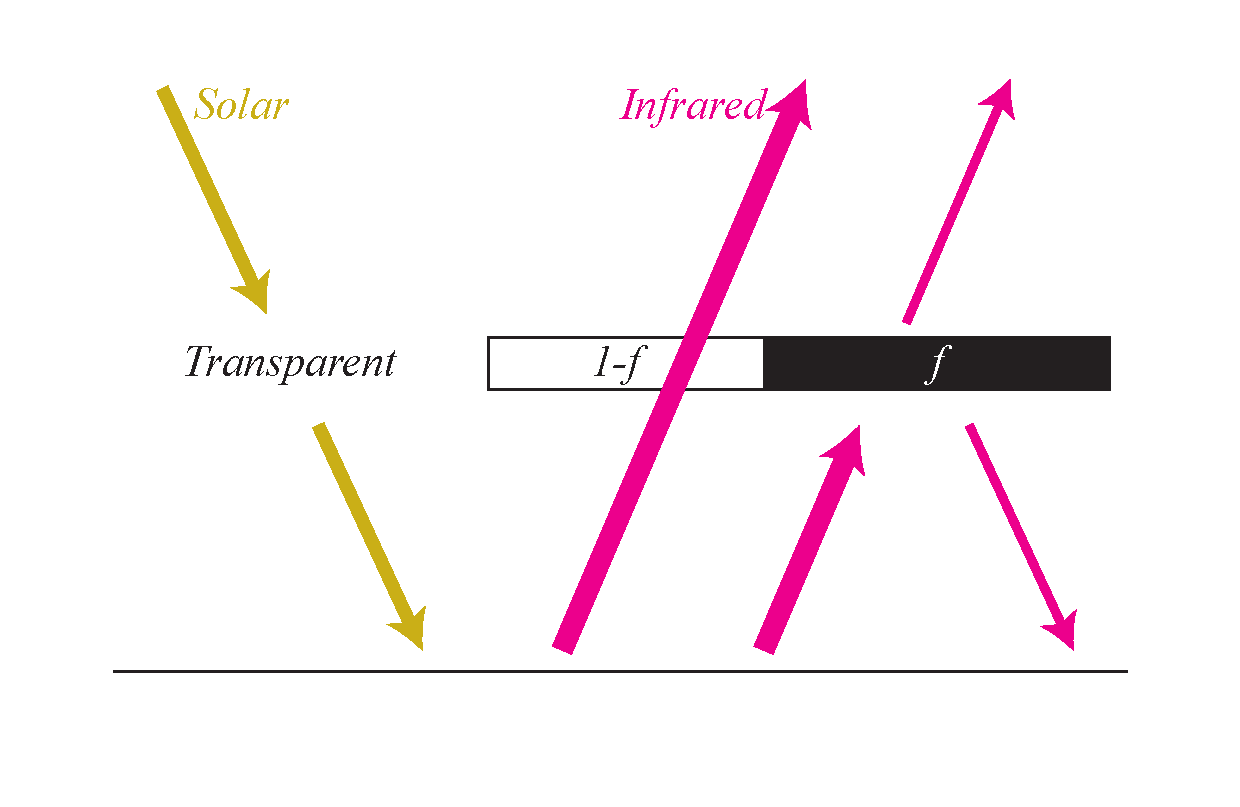
\includegraphics[width=12 cm]{../illustrations/Partially_absorbing_atmosphere}
\end{center}
\caption{ The energy balance for the partially absorbing slab atmosphere.    } 
\label{fig:partially_absorbing_atmosphere}
\end{figure}

Now, let $T_s$ be the surface temperature and $T_a$ be the atmosphere temperature. Unlike in the perfect greenhouse slab case, we cannot assume that the atmosphere temperature equals the emission temperature, $T_e$. We can then set up balances at the top of the atmosphere and at the surface:
\begin{eqnarray}
N_\textrm{toa} &=&  \frac{S_o}{4}(1-\alpha) - f \sigma T_a^4 - (1-f)\sigma T_s^4 \nonumber \\ 
N_\textrm{sfc} &=&  \frac{S_o}{4}(1-\alpha) + f \sigma T_a^4 - \sigma T_s^4 \nonumber 
\end{eqnarray}
Again, we can assume stationarity and solve for $T_s$ and $T_a$:
\begin{equation}
T_s(f) = \sqrt[4]{\frac{S_o(1-\alpha)}{2\sigma(2-f)}}, \ T_a(f) =  \sqrt[4]{\frac{S_o(1-\alpha)}{4\sigma(2-f)}},
\label{eq:partial_absorbtion_solution}
\end{equation}
such that we see that $T_s > T_a$ under all conditions and that they both increase with increasing $f$. For the limit $f \rightarrow 1$ we obtain $T_a \rightarrow T_e$ as in Equation \ref{eq:perfect_greenhouse}, and in the opposite case $f \rightarrow 0$ we obtain $T_s \rightarrow T_e$ as in the ideal black body case of Equation \ref{eq:black_body_energy_balance}. We may also solve for $f$ instead:
\begin{equation}
f = 2 - \frac{S_o(1-\alpha)}{2\sigma T_s^4},
\end{equation}
which for Earth-like conditions gives $f \approx 0.76$, that is, three quarters of the infrared radiation emitted from the surface has to be absorbed by the greenhouse slab if we are to get a surface temperature of 288 K. To obtain balance here, the atmosphere has to be colder than $T_e$, about 242 K. We can understand this as some of the radiation can escape from the surface directly space, so that to obtain energy balance with the incoming solar radiation the atmosphere has to be colder than 255 K such that the average emission temperature is $T_e$. In the limit $f \rightarrow 0$ the atmospheric temperature is about 215 K, but of course, strictly in the limit that temperature looses meaning as no radiation is absorbed and emitted from the atmosphere anymore.


\section{Greenhouse effect of a gaseous atmosphere}
Now in practical cases the atmosphere does not consist of a single, or multiple slabs in radiative equilibrium with the incoming solar radiation and the outgoing infrared radiation, rather it consists of gases, clouds and perhaps some particulate matter. An important property of a gaseous atmosphere is that it is relatively mobile, so that it can overturn and react on timescales comparable to those of radiative heating and cooling. As a first approximation we can think of this by the troposphere having a reasonably fixed lapse-rate with height. For dry mixing this would be about -10 K/km, but as discussed earlier the real atmosphere cools less rapidly with height due to release of latent heat in convective clouds.

\begin{figure}
\begin{center}
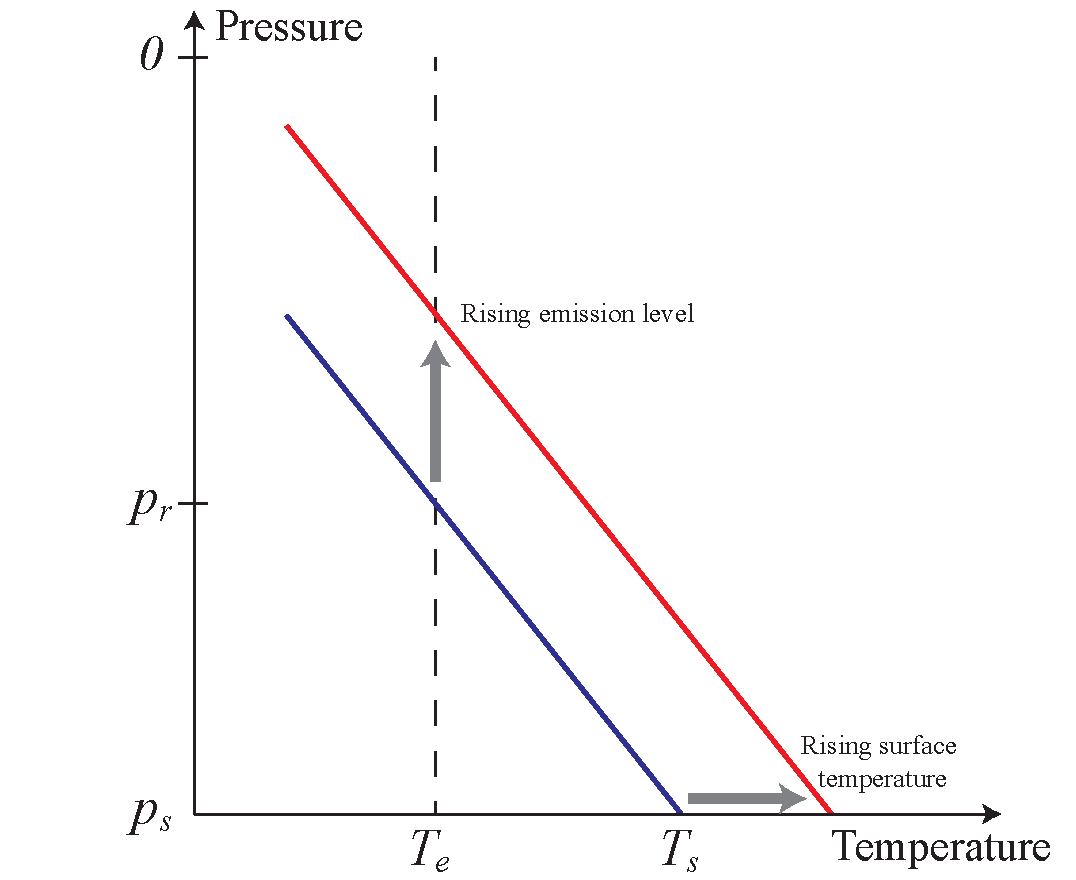
\includegraphics[width=8 cm]{../illustrations/Gaseous_atmosphere_radiation_level}
\end{center}
\caption{ Illustration of the concept of a radiation level pressure for an optically thick atmosphere. With more greenhouse gas (red) the radiation level moves upward and therefore the surface and atmosphere has to warm in order to again radiate as $-\sigma T_e$ to space.   } 
\label{fig:radiation_level}
\end{figure}

Let us start with an atmosphere that is fully transparent to infrared radiation. Here we may think of the Earth's dry atmosphere absent of carbon dioxide, ozone, methane etc. That is, it could for instance consist of nitrogen or oxygen. Then we are effectively having the black body case (Eq. \ref{eq:black_body_energy_balance}) wherein $T_s = T_e$. Then let us add some small amount of a perfect greenhouse gas, one that absorbs equally well at all infrared wavelengths. We shall assume that it is equally distributed everywhere, such as is the case for carbon dioxide (Figure \ref{fig:tropical_profiles}), with a concentration $q$. Trace gas concentrations are fractions typically measured in parts per million (ppm) or parts per billion (ppb).

As we look at this atmosphere from space the radiation emitted towards us is then  a mixture of radiation from different heights. If $q$ is very small some of the radiation emitted by the surface may escape directly to space without being absorbed by the greenhouse gas molecules: some of the photons can slip through, and we call the atmosphere optically thin. In the other limit, if $q$ is large then even a small fraction of the atmospheric column can act as if it was a black body. The pressure thickness of such a layer will scale with the amount greenhouse molecules, $q \Delta p/g$, such that the larger $q$ is, the smaller $\Delta p$ has to be. As we view our optically thick atmosphere from space we will almost exclusively see radiation coming from the uppermost part ($\Delta p$) and it will be characterized by the temperature that prevails in this layer. In this case it may be useful to think of the infrared radiation as coming from a certain radiation level, $p_r < p_s$, that is the height at which the temperature equals the emission temperature, $T_e$. The concept is illustrated in Figure \ref{fig:radiation_level}.

As we add more greenhouse gas to our atmosphere then the pressure thickness, $\Delta p$, required to act as a black body decreases, and so with it $p_r$ becomes smaller. Therefore the emission level moves upward in the atmosphere to lower pressure. But since the emission temperature, $T_e$, is constrained to be that which closes the energy budget of the planet (in the case of Earth $T_e \approx 255$ K) then the whole atmosphere as well as the surface has to warm up. This is because the surface and atmosphere are dynamically coupled by mixing processes to follow closely a certain lapse-rate.

In a nutshell, the reason there is a greenhouse effect is that the atmosphere absorbs some of the radiation emitted by the surface and re-emits at a lower temperature to space. To achieve this the atmosphere has to be colder than the surface; something which is ensured through convective mixing.

% ROUND OFF with a section arguing that greenhouse gases cause greenhouse effect if the atmosphere is colder than the surface and further that greenhouse gases, by cooling the atmosphere, ensure this to happen.


\section{A note on signs}
As you may have already noticed, throughout this set of notes I will count all fluxes as positive downwards. This has the advantage that positive fluxes will act to warm- and negative fluxes cool the system. Likewise, the feedback parameter that we shall define in the next chapter is automatically negative for stable climates and positive for unstable climates. The downside is that the {\em outgoing longwave radiation} emitted by the Earth (OLR) is then a negative flux -- where possible I shall denote it {\em net longwave radiation} trying to avoid confusion. Also note that some figures that I borrow can use the definition where OLR is positive. In the literature a number of sign conventions have developed, and it is worth paying close attention when reading on.

%\newpage
\vspace{1 cm}
{\setlength{\parindent}{0cm}
\hrule
\begin{exercise}
Show that the energy balance for the gray body case leads to this expression of the equilibrium surface temperature:
\begin{equation}
T_s = \sqrt[4]{\frac{S_o(1-\alpha)}{4\epsilon\sigma}}.
\label{eq:gray_radiation}
\end{equation}
Do this by modifying Equation \ref{eq:black_body_energy_balance} replacing $\sigma T_e^4$ with $\epsilon \sigma T_s^4$, where $\epsilon$ is the emissivity. Compare the result with the partially absorbing atmosphere, Equation \ref{eq:partial_absorbtion_solution}, and find out how $\epsilon$ depends on $f$. How small can $\epsilon$ be for a single slab atmosphere? And for $n$ slabs? Estimate the Earth's effective emissivity by solving Equation \ref{eq:gray_radiation} for $\epsilon$.
\end{exercise}

\begin{exercise}
Derive Equation \ref{eq:ntwo} for a two-layer atmosphere in the same way as done for the case for the single-layer atmosphere.
\end{exercise}

\begin{exercise}
Make sure you have access to a computer with Python, and follow the instructions on the handed out sheet.
\end{exercise}

}

%---------------------------------------------------------------------
\chapter{Response to small perturbations}
\vspace{1 cm}

Up until now we considered climates that were stationary, at balance between the absorbed solar radiation and the emitted infrared radiation. We call this a stationary state or a fix-point. But what happens if the system is starting a bit away from that stationary state? Or what happens if we take a system in a stationary state and somehow force it in a way that causes an energy imbalance to occur? This naturally leads us to develop the concepts of radiative forcing, climate change feedbacks and a resulting equilibrium climate sensitivity.
In this chapter we shall assume the perturbations are small such that we can linearize the system.  A surprisingly large part of the discussion around climate change is actually limited to this first-order linear regime and so it makes sense to spend some time on it. In a later chapter we shall explore systems wherein linearity can no longer be assumed and the associated concepts begin to fall apart.

\begin{figure}
\begin{center}
\includegraphics[width=15 cm]{../external_figures/Paleo_temperature_timeseries}
\end{center}
\caption{ Concatenation of various proxies of temperature from the past for illustration purposes. Note the logarithmic time-axis. Modified from the original by Glen Fergus. } 
\label{fig:Paleo_temperature_timeseries}
\end{figure}


\section{Climate stability}
In one perspective the Earth's climate has varied in rich ways in the past, in another perspective it has been remarkably stable (Figure \ref{fig:Paleo_temperature_timeseries}). The past 6.000 years we have had nearly steady temperatures, a period called the Holocene. These relatively mild conditions, wherein modern human civilization developed, have been rare in the past 1.000.000 years wherein the climate has cycled between longer colder glacial periods interrupted by short interglacials. Before that the Earth was warmer than it is today. For instance during Pliocene CO$_2$ concentrations were close to what they are today, about 400 ppm, and temperatures higher than during Holocene by about 2-3 K. Much earlier, during the Eocene temperatures were warmer, maybe by 10-15 K. These differences on the one hand translated into substantially different conditions for life to unfold on the planet. On the other hand, from a physical point of view the Eocene was merely 5 percent warmer than today, as measured on an absolute temperature scale. 
On this background it makes intuitive sense to think that Earth's climate is stable to small perturbations in the context of it's known history: The system did not venture to completely different states and it did spend enough time to equilibrate at almost any temperature within the range visited since dinosaurs ruled the Earth 65 million years ago (Figure \ref{fig:Paleo_temperature_timeseries}); we shall return to estimating the time-scales for equilibrating in the next chapter. It is worth pointing out though that the mere fact that temperatures did not substantially change over that period does not imply that the Earth is {\em insensitive} to perturbations, rather climate has been relatively constant due to the compensation between a longterm increase in $S_o$ and a simultaneous decrease in atmospheric CO$_2$ as carbon has been buried in fossil sediments. 

\begin{figure}
\begin{center}
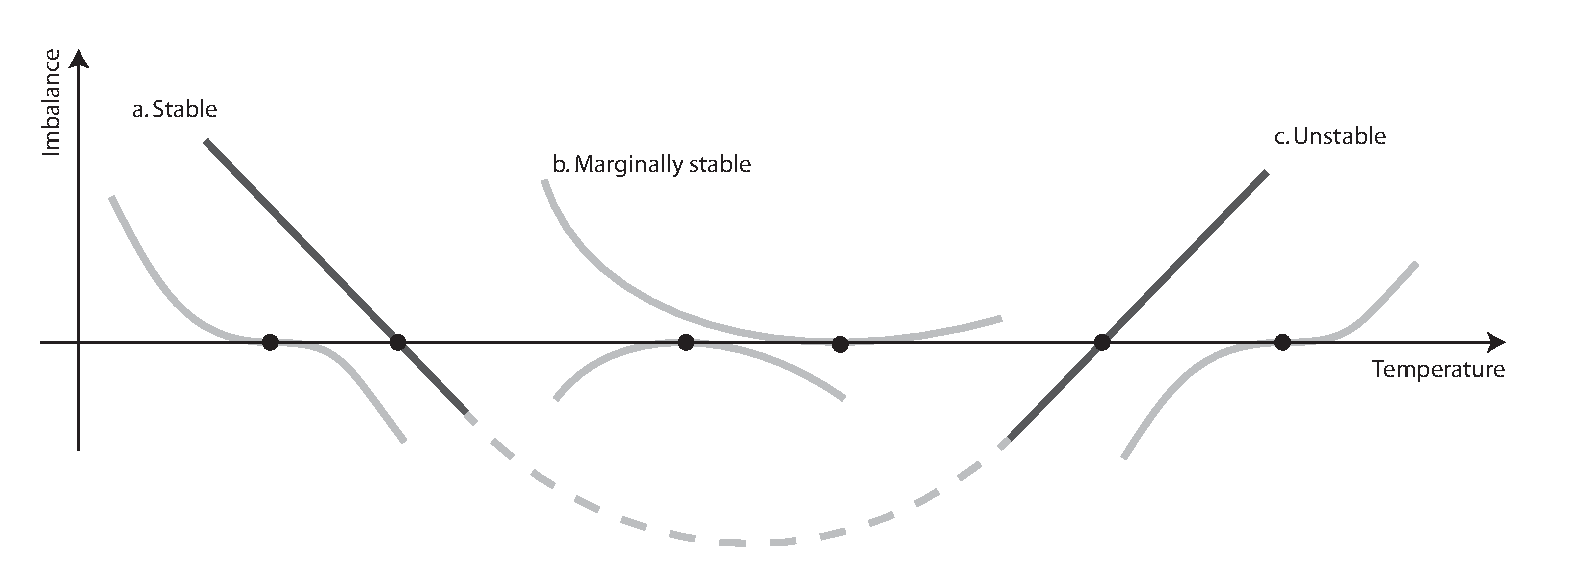
\includegraphics[width=17 cm]{../illustrations/Feedback_stability_cases.pdf}
\end{center}
\caption{ Illustration of stability cases near stationary states as marked by the black dots whereat imbalance is zero. I consider all the light gray cases where $d N/ d T = 0$ at the fix-point as limiting cases. } 
\label{fig:feedback_stability_cases}
\end{figure}

For a state to be stable it must not only have zero imbalance ($N=0$) but it must also be stable to small perturbations. The latter requires that there is some restoring force such that if the system finds itself a bit away from stationarity, then that force will act to move the system back towards the fix-point. We can think of these perturbations as arising due to internal variability, due to weather phenomena or climate variability, or due to external forcing such as fluctuations in the solar constant or changes in atmospheric composition for reasons we consider external to the system, e.g. anthropogenic carbon dioxide emissions. For a complex system such as the Earth's climate this may be difficult to visualize as there is a practically near-infinite number of state-variables. But for many purposes we think of the climate system as having a single state-variable, the global mean surface temperature as we did it in the previous chapter, and in this case we can visualize the problem more easily (Figure \ref{fig:feedback_stability_cases}). In trying to consolidate this one-dimensional view, we may think of all the state variables as being functions of the global mean temperature. 

Now suppose $T_o$ is a fixed-point at which the imbalance is zero and that in {\em some region} above and below $T_o$ the imbalance, $N$, is a continuous and differentiable function of $T$. Then for cases wherein $dN/dT \ne 0$ the fix-points are either stable if $dN/dT < 0$, where the derivative is evaluated at $T_o$, as in some region above $T_o$ the imbalance has to be negative and the system will cool towards $T_o$, and vice-versa if the system is colder than $T_o$ it will warm up again. A similar argument can be made that the system is unstable if $dN/dT > 0$. These two possibilities are displayed as black lines in cases a and c in Figure \ref{fig:feedback_stability_cases}. We shall refer to $dN/dT$ as the feedback parameter ($\lambda$), and the above summarizes that for cases whereat $N(T_o) = 0$ the stability is determined as follows:
\begin{eqnarray}
\lambda(T_o) < 0&:& T_o \textrm{ is a stable fix-point} \nonumber \\� 
\lambda(T_o) > 0&:& T_o \textrm{ is an unstable fix-point} \nonumber
\end{eqnarray}
which is the take-home message of this section.

We talked above about stability in {\em some region} around a fix-point, but what does that mean? How large does the region have to be? It depends on how large the perturbations considered to be relevant are, if there is a faint risk of approaching another fix-point. If a stable and an unstable fix-point exists in immediate vicinity, such as shown by the dashed line in Figure \ref{fig:feedback_stability_cases}, then the stable solution is only stable to small perturbations. If it is pushed hard to temperatures above those of the unstable fix-point, then it will not return to the stable fix-point, but instead continue to warm because there $N>0$. Eventually, the system may then encounter another stable fix-point and settle at warmer temperatures. 

In the rare limiting cases wherein both $N=0$ and $dN/dT = 0$ at the fix point things get a bit more complicated. In this case it makes sense to evaluate $N$ on either side of the fix point. If $N>0$ at somewhat colder $T$ and $N<0$ at slightly warmer $T$ then the system is stable to small perturbations, as illustrated for the gray case a in Figure \ref{fig:feedback_stability_cases}. The same argument can be used for the limiting unstable case, c. In the marginally stable cases (b) wherein $N$ has the same sign on either side of the fix-point the system is stable to perturbations in one direction and unstable to perturbations in the other direction. Think of yourself as standing on a small plateau on the side of a slippery cliff. If you try to climb up the mountain you will slide back towards the plateau (stable), but if you move a bit in the other direction you fall off the cliff and never get back to your starting point (unstable). Marginally stable fix-points occur when a system undergoes so-called bifurcations, a topic we shall return to in a later chapter.

Now let us be more concrete in applying the stability criterion we derived above. We will start with a version of the energy balance equation that you developed in an exercise of the previous chapter. In this case the greenhouse effect is represented by an effective emissivity, $\epsilon$, which is less than or equal to unity:
\begin{equation}
N = \frac{S_o}{4}(1-\alpha) - \epsilon \sigma T_s^4,
\end{equation}
from which we can estimate the feedback parameter by taking the derivative yielding:
\begin{equation}
\lambda = -\frac{S_o}{4}\frac{d\alpha}{dT_s} - \sigma T_s^4 \frac{d\epsilon}{dT_s} - 4 \epsilon \sigma T_s^3,
\label{eq:lambda_general}
\end{equation}
in the general case where $\epsilon$ and $\alpha$ are dependent on temperature. We can think of the first term as shortwave feedback which arises due to changes in planetary albedo. The origin of such feedbacks could be changes in surface albedo, e.g. through the melting of bright snow and ice, or through changes in the cloudiness and water vapor. The two other terms are infrared or longwave feedbacks. The middle term encapsulates changes in the Earth's emissivity with temperature, as we shall see e.g. due to increasing water vapor and rising upper-level clouds with warming. The last term is what is often referred to as the Planck feedback parameter.

If we consider a system with constant $\epsilon$ and $\alpha$ then the only term remaining is the Planck feedback for which we have:
\begin{equation}
\lambda_P = - 4 \epsilon \sigma T_s^3 < 0 
\label{eq:lambda_planck}
\end{equation}
for all $T_s$ implying that this system is unconditionally stable. If we insert numbers typical for the Earth we obtain obtain $\lambda_p \approx$ -3.25 Wm$^{-2}$K$^{-1}$ which is surprisingly close to the value obtained from complex climate models, as we shall see later. The second term on the right hand side of equation \ref{eq:lambda_general}, which is broadly to be thought of as water vapor feedback (plus something called lapse-rate feedback), is found in climate models to be about +1.2 Wm$^{-2}$K$^{-1}$, and so is not sufficient to cause instability in current climates. In warmer climates the positive water vapor feedback is thought to increase faster than the negative Planck feedback and so could aid in destabilising the system. Finally, the first term on right hand side of Eq. \ref{eq:lambda_general} is the planetary albedo feedback, which is due to clouds, surface albedo as well as absorption by the atmosphere foremost water vapor. It is left as an exercise to estimate the criterion for instability when considering planetary albedo feedback.

\section{Feedback mechanisms}
Above we calculated the feedback parameter for the general case (Eq. \ref{eq:lambda_general}) and identified three terms, one related to how planetary albedo changes with temperature, one related to how the effective emissivity changes and one which is directly related to the Planck feedback. Now, if we want to go about understanding and quantifying the feedback it is more convenient to make another division. For instance the planetary albedo is controlled by changes in surface albedo, cloudiness and water vapor, as well as some other factors such as aerosol particles and ozone that we shall ignore here as feedbacks. 
As a first step let us divide $\lambda$ into contributions due to changes in temperature, water vapor, clouds and surface albedo:
\begin{equation}
\lambda =  \lambda_T + \lambda_W + \lambda_C + \lambda_A + ...
\label{eq:lambda_linear_sum}
\end{equation}
where there are a number of additional terms due to interactions between e.g. clouds and water vapor changes as well as other factors that we have ignored. As long as we consider relatively small perturbations  then the interactions between feedbacks are of secondary importance. For large perturbations, however, it is easy to appreciate that this will no longer be the case. For instance at high latitudes cloudiness tends to increase in a warming climate, and so a decreasing surface albedo will have less of an impact on the energy imbalance than in a colder case. Or if the vertical temperature structure is substantially altered due to a rising tropopause, then the impacts of clouds and water vapor changes on the greenhouse effect may be different.
\begin{figure}
\begin{center}
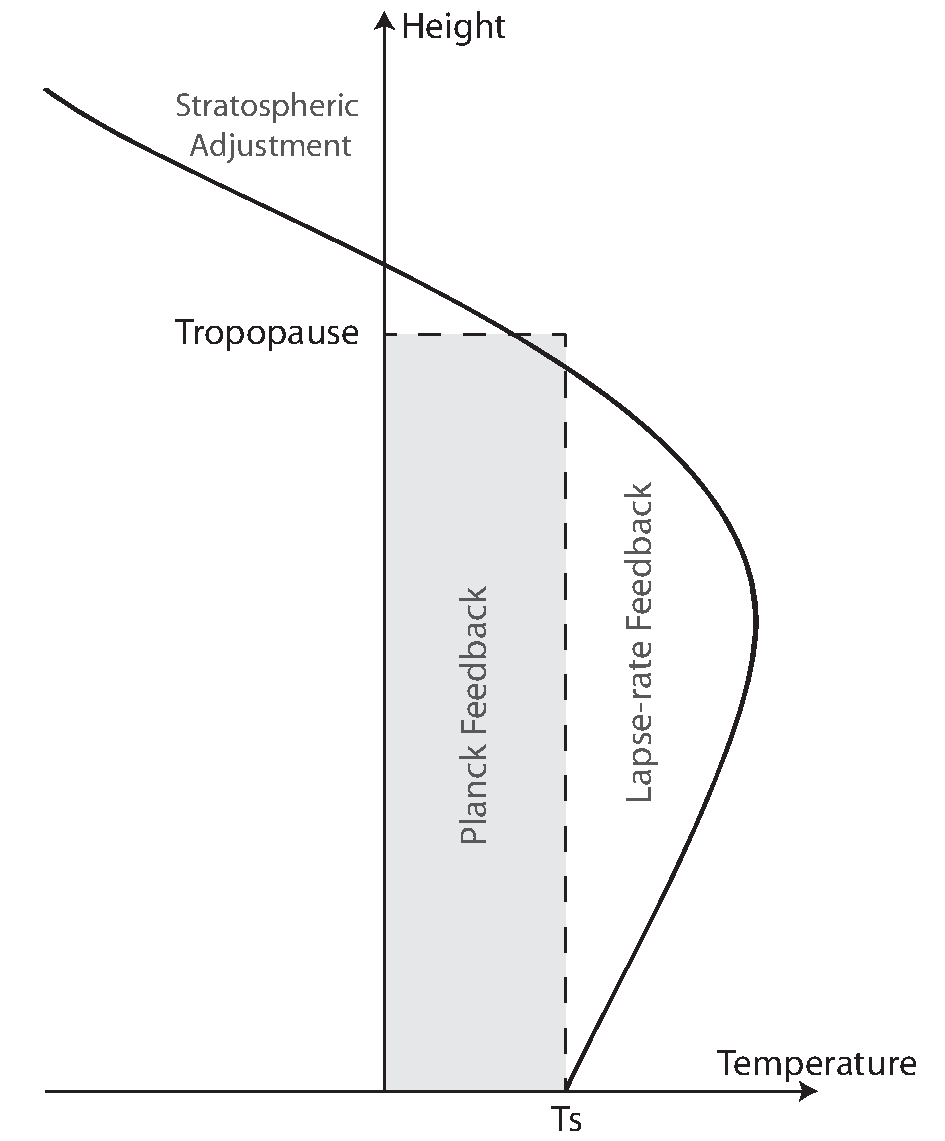
\includegraphics[width=8 cm]{../illustrations/Planck_LR_feedback.pdf}
\end{center}
\caption{ Principle of dividing temperature feedback into two contributions from Planck and Lapse-rate feedback. The shown temperature profile is typical of the tropics; at high latitudes the surface may warm faster than the troposphere. } 
\label{fig:planck_LR}
\end{figure}

It turns out to be meaningful to divide the temperature feedback parameter into two contributions (Figure \ref{fig:planck_LR}). The Planck feedback is that which would occur if the entire troposphere would warm at the rate of the surface temperature (gray shading). The lapse-rate feedback is that due to deviations from vertically uniform warming. In a later chapter we shall study stratospheric adjustment as a response to changing CO$_2$ which is not considered a feedback, and so ignoring the stratospheric temperature changes, we can write the temperature feedback as:
\begin{equation}
\lambda_T \approx \lambda_P + \lambda_{LR}.
\end{equation}
The planck feedback is therefore always negative, whereas the lapse-rate feedback could be either positive or negative: If the troposphere warms faster than the surface temperature then the system can radiate more to space relative to the case where warming was vertically uniform. This is the case in the tropics where the troposphere is vertically mixed by deep convective clouds (as in Figure \ref{fig:planck_LR}). At high latitudes, however, the surface may well warm faster than the troposphere such that the lapse-rate feedback is a positive feedback mechanism acting to amplify regional warming (Pithan and Mauritsen�\cite{Pithan2014}). However, because the tropics cover a much larger area the lapse-rate feedback is thought to be on average negative.

It is worth noting that the division of feedback parameters chosen here is only one of many possible divisions, a few of which makes sense. A powerful recent development has been to include some of the water vapor feedback into the temperature feedback, namely that which would occur if relative humidity stayed fixed (Held and Shell\cite{Held2012}). This is effective since, as we shall argue next, changes in relative humidity tend to be small in climate models. 

Complex climate models agree broadly on the importance of these feedback mechanisms, although the strengths of feedback parameters are model dependent. Table \ref{table:feedbacks} shows a dozen examples from some of the models that participated in the fifth phase of the Coupled Model Intercomparison Project (CMIP5). In particular the cloud feedback parameter varies substantially among models. An example of the spatial patterns of the feedback parameters is shown for one climate model in Figure \ref{fig:feedback_maps}. We see that the temperature feedbacks are the dominant negative feedback, whereas water vapor feedback is generally positive and strongest in the moist tropical regions. Surface albedo feedback is positive in regions were snow and sea ice melts. Finally, cloud feedbacks exhibit complex patterns which are different from model to model. Next we shall look at a some of the individual feedback mechanisms.

\begin{table}
  \caption{ Overview of feedback parameter strength (Wm$^{-2}$K$^{-1}$) in some climate models as diagnosed using the radiative kernel method. The cloud feedback parameter is split into shortwave ($\lambda_{C,SW}$) and longwave ($\lambda_{C,LW}$) contributions, and I also provide the sum of water vapor and lapse-rate feedback ($\lambda_{W+LR}$). This is a subset of the analysis from Caldwell et al.\cite{Caldwell2016}. }
  \vspace{0.5 cm}
  \centering
  \begin{tabular}{l|rrrrr|rr|r} 
Model                 & $\lambda_P$ & $\lambda_{W}$ & $\lambda_{LR}$ & $\lambda_{C}$ & $\lambda_A$ & $\lambda_{C,SW} $ & $\lambda_{C,LW}$  & $\lambda_{W+LR}$  \\
\hline
ACCESS1.3&	-3.16	&1.65&	-0.49&0.68&	0.39&	0.53&	0.15&	1.16 \\
BNU-ESM	& 	-3.08&1.46&	-0.17	&0.24&	0.56&	-0.12	&	0.36&	1.29 \\
CCSM4&	         -3.14&1.47&	-0.29	&0.27&	0.43&	0.00&	0.27&	1.18 \\
CanESM2& 	-3.22	&1.77&	-0.49	&0.54&	0.36&	-0.24	&	0.78&	1.28 \\
FGOALS-g2&	-3.15	&1.52&	-0.22	&0.39&	0.54&	0.00&	0.39&	1.30 \\
GFDL-CM3&	-3.12	&1.67&	-0.64	&0.92&	0.40&	0.64&	0.28&	1.03 \\
HadGEM2-ES&	-3.13	&1.62&	-0.41	&0.73&	0.35&	0.31&	0.42&	1.21 \\
IPSL-CM5A-LR	&-3.19&2.02&	-0.94	&1.17&	0.23&	0.63&	0.54&	1.08 \\
MIROC5& 	-3.19	&1.86&	-0.67	&0.00&	0.42&	-0.32	&	0.32&	1.19 \\
MPI-ESM-LR&	-3.10	&1.80&	-0.80	&0.46&	0.39&	-0.14	&	0.60&	1.00 \\
MRI-CGCM3&	-3.19	&1.49&	-0.34	&0.30&	0.45&	0.30&	0.00&	1.15 \\
NorESM1-M&	-3.11	&1.48&	-0.23	&0.35&	0.39&	0.07&	0.28&	1.25 \\
INM-CM4.0&	-3.11	&1.59&	-0.43	&0.23&	0.38&	0.01&	0.22&	1.16 \\
\hline								
Ensemble mean&	-3.15&	1.65&	-0.47&	0.48&	0.41&	0.13&	0.35&	1.18 \\
Standard deviation&	0.04&	0.17&	0.24&	0.32&	0.08&	0.32&	0.20&	0.10
  \end{tabular}
  \label{table:feedbacks}
\end{table}



\begin{figure}
\begin{center}
\includegraphics[width=15 cm]{../external_figures/MPI-ESM_abrupt4xCO2_allfeedbacks_contour.png}
\end{center}
\caption{ Maps of feedback from MPI-ESM-LR, from Block and Mauritsen \cite{Block2013}. } 
\label{fig:feedback_maps}
\end{figure}

\subsection{Surface albedo feedback}
Perhaps the simplest feedback to comprehend is the surface albedo feedback. That is, at least the more important parts of the feedback that are related to melting snow and sea ice -- changes in vegetation may also impact the surface albedo -- and at least as long as we are thinking about a small warming relative to the present climate. In a later chapter we shall look at what happens if we instead cool the system and it might enter a snow-ball instability. 

\begin{figure}
\begin{center}
\includegraphics[width=12 cm]{../plots/CERES_Ebaf_shortwave.pdf}
\end{center}
\caption{ Shortwave fluxes observed and inferred from the CERES dataset. Black is the downwelling annually averaged sunlight at the top of the atmosphere, on average 340 Wm$^{-2}$. The red line is the downwelling sunlight at the surface (187 Wm$^{-2}$), and the blue is the reflected sunlight at the surface (24 Wm$^{-2}$). Therefor the gray shaded area is the surface absorption. Over the region poleward of 60N the corresponding three numbers are 201, 102, 43 Wm$^{-2}$, respectively. } 
\label{fig:CERES_shortwave}
\end{figure}

So let us focus on the Arctic region, where most of the surface albedo feedback occurs with respect to warming (Figure \ref{fig:feedback_maps}). As a first attempt at constraining this feedback, let us assume there is no atmosphere and therefore also no clouds. Thus all incoming radiation arrives at the surface, and a fraction $A$ is reflected back to space. Suppose the surface albedo changes by an amount $\Delta A$ for a global warming of $\Delta T$ and let $S$ be the incoming solar radiation. Then regionally the imbalance changes by an amount $S \Delta A / \Delta T$. On average over the region poleward of 60N $S=201$ Wm$^{-2}$ (Figure \ref{fig:CERES_shortwave}). Complex climate models have that most of their Arctic sea ice is gone at a global mean temperature around 20$^\circ$C (currently about 15$^\circ$C), so $\Delta T \approx 5$ K. The observed average effective surface albedo in the region is 0.42 (Figure \ref{fig:CERES_shortwave}), which would then drop to about 0.07 which is that of an open ocean. The area of a spherical cap is $2\pi r^2 (1-\sin\theta)$, where $\theta$ is the angle from the Equator to the pole, whereas we recall the surface area of the whole Earth is $4\pi r^2$. Thus, suppose we consider the region poleward of 60N then that is little less than 7 percent of the Earth's surface; if we restrict this to mainly be the Arctic ocean roughly poleward of 70N then it is only 3 percent of the Earth. Then we can estimate an upper bound on the contribution of the Arctic region to global surface albedo feedback parameter as:
\begin{equation}
\frac{\textrm{polar cap area}}{\textrm{global area}} \cdot \frac{\Delta A} {\Delta T} \cdot S \approx 1.0 \ \textrm{Wm}^{-2}\textrm{K}^{-1}.
\end{equation}
Now this is a gross overestimate. The reason is that the atmosphere, which we neglected above, hinders (absorbs or reflects) roughly half of the radiation at the top of the atmosphere from reaching the surface in the Arctic region. This alone would half the surface albedo feedback parameter. But the surface reflected sunlight would have to, once again traverse the atmosphere before escaping to space, whereby again about half the radiation would be either reflected back towards the surface or absorbed by the atmosphere. Accounting for this would leave us with a quarter of the original estimate, or roughly $\lambda_A \approx 0.25$ Wm$^{-2}$K$^{-1}$ originating in the Arctic region only. Other regions, e.g. the Southern Ocean, also contribute to the surface albedo feedback making the climate model ensemble mean global $\lambda_A \approx 0.41$ Wm$^{-2}$K$^{-1}$ seem plausible (Table \ref{table:feedbacks}). The calculation shows that in addition to how fast the regional surface albedo changes with global warming, perhaps the most important factor in determining the surface albedo feedbacks is the attenuation of sunlight by the atmosphere, which in turn is mostly dependent on cloudiness at these high latitudes.


\subsection{Water vapor feedback}
As we saw in the beginning of the course, water vapor is an excellent greenhouse gas in that it absorbs across a wide range of the infrared spectrum. A problem with water vapor is that, unlike CO$_2$, it is highly inhomogeneously distributed in the atmosphere both vertically, horizontally and in time; in Figure  \ref{fig:tropical_profiles} we saw how the average mixing ratio of water vapor in the tropics changes a factor 10.000 from the surface to the tropopause. This is because the lifetime of a water vapor molecule in the troposphere is relatively short, about a week or so, before it is for the most part precipitated out. The maximum amount of water vapor the atmosphere can hold before it starts condensing into cloud droplets is highly temperature dependent, roughly exponential according to the Clausius-Clapeyron relationship. 

\begin{figure}
\begin{center}
\includegraphics[width=14 cm]{../external_figures/RH_change_echam-6_3_02p4_amip4K_zonalmean.png}
\end{center}
\caption{ Change in relative humidity in a model experiment where the ocean surface temperature is raised uniformly by 4 K.} 
\label{fig:RH_change_ECHAM}
\end{figure}

Fortunately, we can argue that relative humidity ($RH$) stays approximately constant under climate change. Relative humidity is the actual water vapor pressure ($e$) relative to the saturation vapor pressure ($e_s$). For the argument we will be making it is perhaps easier to think of the water vapor mixing ratio which is conserved with adiabatic motion ($q$, such that $RH \approx q/q_s$). If we trace an isolated air parcel along it's trajectory through the atmosphere we will find that it spends part of its time being saturated within clouds and part of its time being sub-saturated in clear air. As long as it is inside clouds it will have $q=q_s$, and so too at the exact moment the parcel leaves the cloud. Let us call this $q_s(T_c)$ where $T_c$ is the temperature at the last contact with cloud. Subsequently, in the cloud-free part of the parcels trajectory, where by necessity $T \ge T_c$, the water vapor mixing ratio at the last contact with cloud is conserved and so the relative humidity is $RH = q_s(T_c)/q_s(T) \le 1$. 

We can think of the total atmospheric circulation as consisting of many such trajectories of small parcels of air, each undergoing cloudy and cloud-free transects. Now, suppose the atmospheric circulation stays unchanged in a statistical sense under small amounts of climate change, then the only thing that changes for our parcels is the temperatures at which they operate. If then the entire troposphere warms at about the same rate, then for a given trajectory both $T_c$ and $T$ change by the same amount and so to first order $RH$ stays constant under climate change. To investigate how good an approximation this is, I plotted the change in $RH$ in Figure \ref{fig:RH_change_ECHAM} as the difference between two experiments: one with sea-surface temperatures prescribed as observed and one wherein I added a horizontally uniform warming of 4 K. In most of the troposphere the changes in $RH$ is less than or around 1 percent per Kelvin warming. In the tropopause and lower stratosphere region there is a substantial rise in $RH$, in part associated with a rise of the tropopause as discussed in the first chapter.

With this result at hand we can now estimate how the specific humidity changes with warming. Our starting point is the Clausius-Clapeyron relation for the saturation vapor pressure:
\[ \frac{de_s}{dT} = \frac{L}{R_v T^2} e_s, \]
which can be rewritten as:
\begin{equation}
\frac{d\ln e_s}{dT} = \frac{L}{R_v T^2},
\label{eq:clausius_clapeyron}
\end{equation}
such that the fractional rate of change of the saturation vapor pressure is a simple function of temperature. $L$ denotes the latent heat of evaporation (about $2.5 \cdot 10^6$ J kg$^{-1}$) and $R_v$ is the gas constant for water vapor (about $461$ J kg$^{-1}$ K$^{-1}$). Inserting different temperatures on the right hand side of Equation \ref{eq:clausius_clapeyron}, one finds that near the Earth's surface one finds increases of 6-8 percent per degree warming, and for tropical upper-tropospheric temperatures around 14 percent per degree warming. Since most of the water vapor resides in the lower troposphere the water vapor path scales with close to 7 percent per degree warming.

The reader is reminded that the infrared part of the water vapor feedback only works because the atmosphere is colder than the surface. Thus adding a water vapor molecule to the atmosphere near the surface is less effective than adding it near the tropopause, and so despite the amount of water vapor in the upper troposphere is much smaller than near the surface it still plays an important role in controlling the infrared radiation to space. The troposphere is colder than the surface in most places and at most times. 
An exception where the atmosphere can be warmer than the surface occurs at high latitudes in winter, and so there raising the emissivity of the atmosphere by adding water vapor will result in more infrared radiation escaping to space. 
A not negligible part of the water vapor feedback of about 20-30 percent, however, occurs because water vapor absorbs sunlight. This absorption depends less on where in the vertical the water vapor is, and more on the column integrated amount, the latitude and season, as well as the presence of clouds and the reflectivity of the surface.
It is left as an exercise to estimate the infrared part of the water vapor feedback under the assumption of constant relative humidity using the MODTRAN model and compare the result with that of more complex climate models. 

% Show a figure with Clausius-Clapeyron, argue that the warming of parcels moving from the upper troposphere to the lower is larger in a warmer climate, hence a slight reduction in RH

\subsection{Cloud feedbacks}
Clouds are exceptionally complicated, and I would be foolish to even try to account for the many different ways in which clouds could possibly feed back on the Earth's energy balance. And not only are the mechanisms complex and difficult to grasp, they are also the main source of uncertainty in quantifying climate change and clouds impact the strength of other feedback mechanisms as we have seen above in the example of surface albedo feedback. Therefore, cloud feedbacks are very much central to the part of climate sciences that aims at estimating Earth's climate sensitivity. Because it is so complicated, one current trend is to dissect the cloud feedback into separate regimes (Figure \ref{fig:cloud_feedback_illustration}) wherein the hope is that the individual mechanisms can be understood and quantified. It is not at all clear that this is the most effective way to achieve overall progress, though, and climate scientists also pursue other routes to determining feedback. 
Current thinking is that it is useful to divide cloud feedback into three groups:
\begin{itemize}
\item Mid- to high latitude mixed-phase clouds
\item Low-level clouds 
\item Deep clouds,
\end{itemize}
although one could certainly think of other divisions that would be meaningful. The first two categories act mostly in the shortwave bands by regulating the planetary albedo, whereas the third category is thought to mainly function in the longwave by regulating the infrared radiation emitted to space.

\begin{figure}
\begin{center}
\includegraphics[width=17 cm]{../illustrations/Cloud_feedbacks_illustration.png}
\end{center}
\caption{ Illustration of various cloud feedback mechanisms. To the left is mixed-phase cloud feedback occurring at mid- to high latitudes in for instance frontal clouds, in the lower middle I show several mechanisms related to low-level stratocumulus and trade-wind cumulus cloud feedbacks, and to the right are deep cloud feedbacks which are thought to act mainly by regulating the infrared radiation escaping to space. } 
\label{fig:cloud_feedback_illustration}
\end{figure}

Ice clouds are generally less reflective to sunlight than are liquid clouds. This is primarily because ice crystals tend to be few and large, whereas cloud droplets tend to be small but many: the cross-section of many small droplets is larger for a given amount of condensate. In a warming climate the isotherms will move upward in the atmosphere and poleward alone resulting in a larger fraction of liquid clouds (Figure \ref{fig:cloud_feedback_illustration}), and so a negative shortwave cloud feedback must result. 
If all clouds at temperatures below the melting point (0$^\circ$C), then a very strong negative feedback would result. However, it is a bit more complicated. At temperatures above 0$^\circ$C all clouds consist of the liquid phase, and below about -35$^\circ$C all clouds consist of ice phase. Between these temperatures both phases can exist, we say clouds are of mixed phase. The more one can maintain liquid clouds at temperatures below the melting point, the weaker the mixed-phase feedback is as there is simply less ice clouds that can be transformed.
Signs of what might be dominating negative mixed-phase cloud feedback can be seen in the Southern Ocean, North Pacific and the Arctic in the MPI-ESM-LR model (Figure \ref{fig:feedback_maps}). This is not the only type of cloud feedback in those regions though, and for instance total cloud feedback appears to be positive in the North Atlantic, a region where we would also expect mixed-phase cloud feedback to be active. A couple of recent studies try to observationally constrain mixed-phase feedback. One study finds that complex climate models are on average correct, with some models having stronger and some models having weaker feedback. Another study finds that models as a whole overestimate the strength of the negative mixed-phase cloud feedback.

Low-level clouds in the tropics and sub-tropics on the contrary consist mostly of liquid droplets. They are, nevertheless, consistently identified as the main source of spread in complex climate model feedback, which is likely due to there being a large number of competing mechanisms (Figure \ref{fig:cloud_feedback_illustration}), explaining all of which I couldn't possibly do any justice here. Foremost, the low-level clouds may regulate the planetary albedo either by changing their coverage or by changing their reflectivity. The reflectivity of low-level clouds is mainly controlled by the amount of condensate. We saw previously that in a warmer climate the atmosphere holds more water vapor, as of Clausius-Clapeyron, and so a naive expectation is that low-level clouds will thicken as there is more vapor to condense (adiabatic thickening). Counteracting this, is the mixing of the moist lower atmospheric air with dry air subsiding from aloft: in a warmer climate the difference in specific humidity will be larger between the boundary layer and the subsiding air, and so the mixing down of air (entrainment) results in a larger depression of relative humidity and fewer clouds in a warmer climate. The strength of the mixing, in turn, is controlled by the strength of the temperature inversion above the boundary layer. In some regions of the sub-tropics this inversion is expected to strengthen in a warmer climate resulting in more cloudiness. Overall, complex climate models can exhibit both positive and negative low-level cloud feedbacks, but there is a tendency for observational and fine-scale cloud modeling evidence to favor positive feedback from this regime.

\begin{figure}
\begin{center}
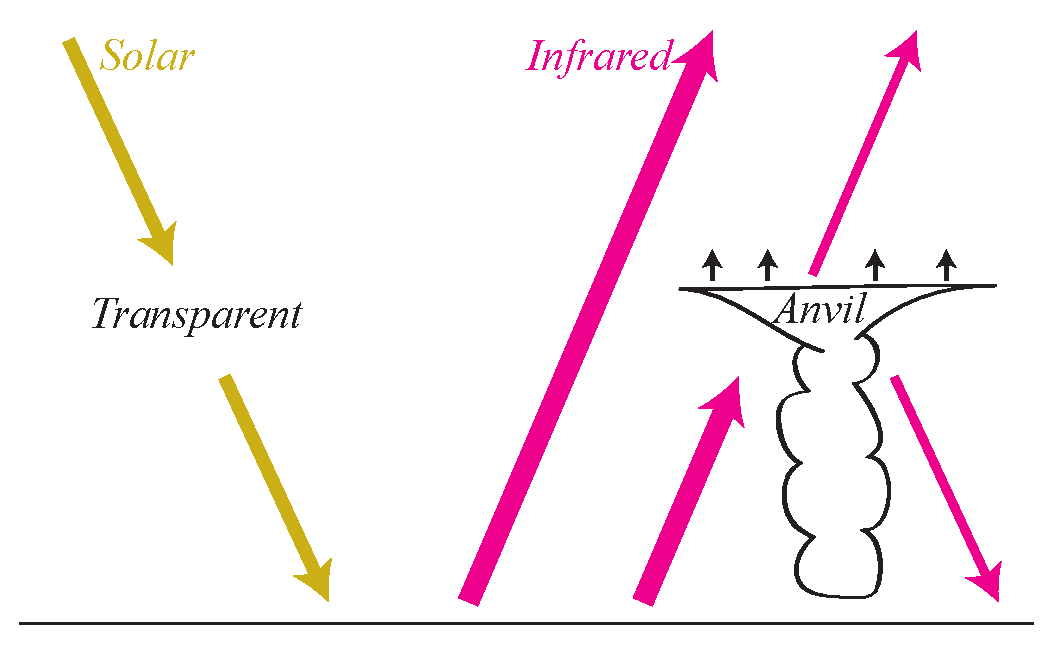
\includegraphics[width=10 cm]{../illustrations/Deep_cloud_feedback_illustration.pdf}
\end{center}
\caption{ Illustration of the infrared feedback from deep clouds. The upper level clouds are thought to move upward in a warming climate so as to maintain a nearly constant temperature of about 200 K, alone resulting in the positive fixed-anvil temperature feedback. There may also be changes in the anvil coverage, something which is popularly denoted iris-effect. } 
\label{fig:deep_cloud_feedback_illustration}
\end{figure}

Deep cloud feedbacks originate for the most part in the tropical regions. We argued in an earlier chapter that the tropopause might move upward in a warming climate so as to maintain an approximately constant temperature, and with it, presumably also that of the deepest convective cloud tops (anvils). 
To see how this ascendence of upper level clouds might exert a cloud feedback, let us consider the gray body case with an upper-level cloud that covers a fraction, $f$, which acts as an ideal black body. The cloud is assumed to rise such as to maintain a constant temperature with a warming surface ($dT_a/dT_s=0$, Figure \ref{fig:deep_cloud_feedback_illustration}). Since there is only one unknown in our problem, $T_s$, we also only need to form one energy balance equation; we choose the top of the atmosphere:
\begin{equation}
N = \frac{S_o}{4}(1-\alpha) - (1-f) \epsilon \sigma T_s^4 - f\sigma T_a^4.
\label{eq:anvil_balance}
\end{equation}
First, let us assume that $f$ is constant such that the upper level cloud maintains its coverage, then we can calculate the feedback parameter:
\begin{equation}
\lambda =  - 4(1-f) \epsilon \sigma T_s^3,
\end{equation}
where we note that $dT_a/dT_s=0$. Comparing to the Planck feedback parameter, Equation�(\ref{eq:lambda_planck}), we immediately recognize that this can be rewritten as:
\begin{equation}
\lambda =  \lambda_P + f 4 \epsilon \sigma T_s^3,
\end{equation}
where the second term is then the fixed anvil temperature (FAT) feedback parameter. Notice how the actual temperature of the cloud, $T_a$, plays no role in determining the strength of the feedback. Since the FAT feedback parameter equals $-f\lambda_P$ we can readily estimate what $f$ has to be around 0.11 to provide the longwave cloud feedback parameter found in complex climate models ($\lambda_{C,LW}$, Table \ref{table:feedbacks}). The estimate of $f$ is smaller than expected since tropical upper-level cirrus clouds cover a larger fraction of the Earth, perhaps twice as much. However, because they consist of few relatively large ice crystal their longwave emissivity is usually less than unity and so in this more realistic setting it requires a larger coverage to reach the same amount of feedback.

Now, let the area $f$ covered with our upper-level black body cloud vary with temperature to emulate an iris-effect. Now the derivative with respect to $T_s$ of Equation (\ref{eq:anvil_balance}) becomes a bit more complicated:
\begin{eqnarray}
\lambda &=&  \lambda_P + f 4 \epsilon \sigma T_s^3 + \epsilon \sigma T_s^4\frac{df}{dT_s} - \sigma T_a^4\frac{df}{dT_s} \nonumber \\
&=&  \lambda_P + \lambda_{FAT} +  \sigma \left( \epsilon T_s^4 - T_a^4\right)\frac{df}{dT_s},
\label{eq:lambda_iris}
\end{eqnarray}
where we recognize the second term as the FAT feedback parameter. The third term represents a replacement of radiation originating from the upper-level cloud to radiation originating from the surface if $df/dT_s$ is negative. In this extreme example it takes only a 2 percent per degree warming reduction of the anvil coverage ($df/dT_s \approx -0.02f$) for the iris-effect feedback parameter to be as strong as  $\lambda_{FAT}$. This is an underestimate of the amount of reduction required for several reasons. First, if cloud cover decreases then the planetary albedo also decreases, thereby inducing a compensating positive shortwave cloud feedback. Second, most of the upper-level cirrus cloud is optically too thin to act as ideal black bodies, further requiring a larger reduction. Together, I believe it might take around 5 percent reduction per degree warming, or so, to be able to compensate the positive FAT feedback.
Complex climate models exhibit no, or only very weak, reductions of anvil area with warming, whereas different lines of observational evidence suggest that models underestimate this reduction. The interpretation of the data, however, remains contentious and it is also currently not known mechanistically why anvil coverage would reduce substantially in a warming climate.

% Add a figure with Earth's effective emissivity from CERES, also clear sky
% Use this to argue that $f$ is larger because the local \epsilon is much smaller in the deep tropics were convective cloud feedbacks act

\section{Equilibrium climate sensitivity (ECS)}
So far we have been agnostic as to why the climate system might be out of balance. It could be due to some random fluctuation, a short volcanic eruption, a change in the solar constant, or forced by a change in the atmospheric greenhouse gas concentration. We shall return to radiative forcing in more detail later, but a standard way to define the sensitivity of the climate system is to expose it to a doubling of CO$_2$ relative to the pre-industrial level which reduces the infrared radiation to space and yields a top-of-atmosphere imbalance of:
$$F_{2x} \approx 3.7 \ \textrm{Wm}^{-2}.$$
A neat thing about CO$_2$ is that the atmosphere is optically thick in the part of the spectrum dominated by CO$_2$ absorption. This leads to the forcing being almost logarithmic in the concentration so that each doubling (from 1 to 2xCO$_2$, from 2 to 4xCO$_2$ etc.) results in about the same amount of forcing. If we think $F_{2x}$ is a sufficiently small perturbation that the feedback parameter, $\lambda$, can be considered constant then we can write the energy balance equation as:
\begin{equation}
N = F_{2x} + \lambda \Delta T
\end{equation}
where we have linearized around a base state. Imagine that we instantaneously double the CO$_2$ concentration in the atmosphere. At this very moment we have $N=F_{2x}$ and the system will start warming. With the warming ($\Delta T > 0$) feedbacks start acting. If the system is stable ($\lambda < 0$) then the warming will lead to a reduction in the planetary imbalance ($N$). It is quite popular to think of this system as an electric feedback loop circuit (Figure \ref{fig:feedback_illustration}). 

\begin{figure}
\begin{center}
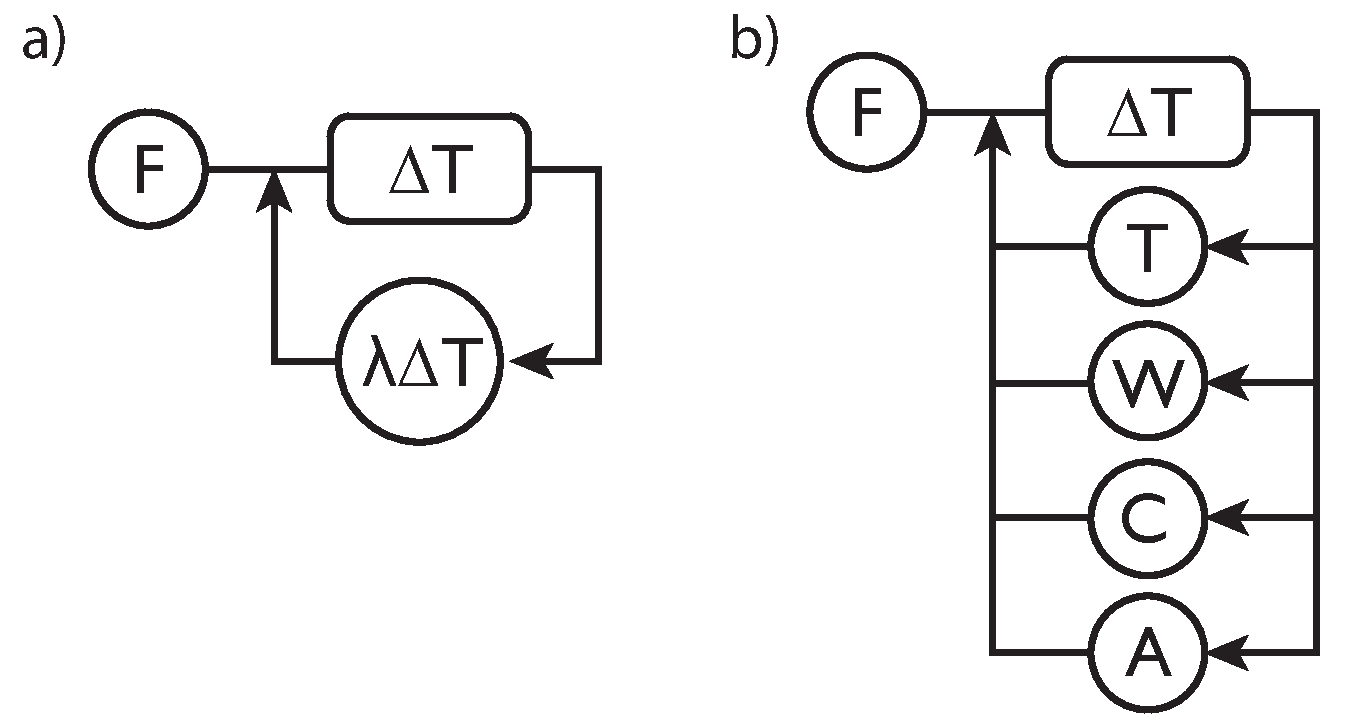
\includegraphics[width=9 cm]{../illustrations/Feedback_illustration.pdf}
\end{center}
\caption{ Illustration of the principle of climate change feedback to external forcing $F$. In case a) the feedback is the product of the total feedback parameter, $\lambda$, and the temperature change. In case b) I divide this into a linear sum corresponding to equation \ref{eq:lambda_linear_sum}, whereby for instance the symbol is $T=\lambda_T \Delta T$. } 
\label{fig:feedback_illustration}
\end{figure}

Eventually, after some time, our system may reach a new equilibrium where $N=0$. Here the temperature change, which we call the equilibrium climate sensitivity (ECS) is:
\begin{equation}
\textrm{ECS} = \frac{-F_{2x}}{\lambda}.
\end{equation}
The inverse relationship between the total feedback parameter ($\lambda$) and ECS is plotted as the black curve in Figure \ref{fig:feedback_vs_ECS} along with estimates from complex climate models. All models exhibit higher sensitivity than what would be the case if there would only be Planck feedback (dashed line). The scatter of models around the theoretical line can have several causes, for instance $F_{2x}$ is model-dependent and there may be non-linearities impacting the estimates. Nevertheless, most of the spread in ECS is due to spread in the total feedback parameter. It is left as an exercise to explore how uncertainty in the strength of feedback mechanisms impact ECS.

\begin{figure}
\begin{center}
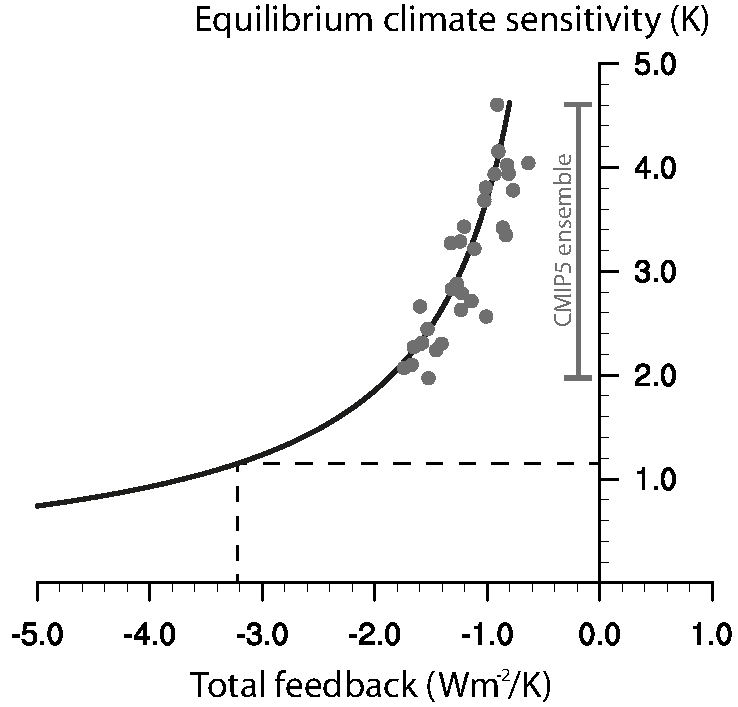
\includegraphics[width=8 cm]{../external_figures/Feedback_vs_ECS.pdf}
\end{center}
\caption{ Relationship between feedback and equilibrium climate sensitivity to one doubling of CO$_2$, ie. a forcing of 3.7 Wm$^{-2}$. Gray dots show individual CMIP5 climate models, and the dashed line indicates the case with only Planck feedback ($\lambda=\lambda_P$). Adapted from Mauritsen and Stevens \cite{Mauritsen2015}.} 
\label{fig:feedback_vs_ECS}
\end{figure}



\newpage
\vspace{1 cm}
{\setlength{\parindent}{0cm}
%\hrule
\begin{exercise}
Estimate the limit of instability for planetary albedo feedbacks using equation \ref{eq:lambda_general}.  Assume here that $\epsilon$ is a constant. Put in numbers relevant for Earth to estimate how fast planetary albedo would have to decrease to alone cause instability.  
\end{exercise}

\begin{exercise}
Calculate the feedback parameter $\lambda = dN/dT_s$ for the partially absorbing slab atmosphere derived in the previous chapter, section \ref{sec:partially_absorbing_slab}. Do so by eliminating $T_a$ from the top-of-atmosphere imbalance equation and then take the derivative with respect to $T_s$. Calculate ECS with reasonable parameters for Earth.
\end{exercise}

\begin{exercise}
Use the online MODTRAN radiative transfer model to estimate water vapor feedback. Do so by changing the 'Water Vapor Scale' from, say, 1.00 to 1.07, corresponding to a 7 percent increase of specific humidity which is roughly what occurs for a 1 K warming at typical tropospheric temperatures. Another way to do this is to use the 'Ground T offset', which actually increases the temperature of the whole column, then compare the cases with constant vapor pressure and relative humidity. It is convenient to use the 'Save this run to background' button.
How does the water vapor feedback depend on locality? How does your estimate compare with that of complex climate models?
\end{exercise}

\begin{exercise}
Estimate the ECS using the complex climate model ensemble mean feedback factors $ \lambda_P + \lambda_{W+LR} + \lambda_C + \lambda_A$ as listed in Table�$\ $�\ref{table:feedbacks}. Note that you are to use the sum of the water vapor and lapse-rate feedbacks. What happens to ECS if each feedback is one standard deviation larger, respectively, smaller? Repeat the calculations without cloud feedback. 
\end{exercise}

}


%---------------------------------------------------------------------
\chapter{Temporal evolution}

In the previous chapter we focussed on the stability of stationary states and the equilibrium response to a small forcing. Here we will investigate how the system approaches these equilibria and how it responds to forcing. This involves considerations of the relevant heat reservoirs, and ignorance of those that do not matter. On this background we will develop a mixed-layer and a two-layer model and study their behavior. 

\section{Heat capacities}
When we think of the Earth's climate system there are several components that can absorb energy with different heat capacities and with different timescales involved. Usually we think of the oceans as the largest component followed by the atmosphere and cryosphere. There are, however, parts of these components that are closely connected to the surface temperature, and there are parts that are weakly connected to the surface. This means, foremost, that it is meaningful to divide the oceans into two or more parts.

If we start with the atmosphere, we saw in the first chapter how the troposphere is for the most part quickly stirred, mixed or overturned by various motion. Therefore it does not take very long for air to be mixed around the world, roughly on the order of months, though the time it takes to cross the equator can be longer. The stratosphere in turn, we found was in radiative equilibrium and stable stratified; though it isn't motionless. There are quite strong zonal winds, and also there is an overturning circulation called the Brewer-Dobson circulation. The latter starts at the tropical tropopause with upward motion, goes up, poleward and terminates in the high latitudes. It takes, however, on the order of five years. The atmosphere weighs in at nearly 10.000 kg m$^{-2}$, which corresponds to the hydrostatic surface pressure of 98.500 Pa, or about that of a column of 10 meters of liquid water. The specific heat capacity of air is, however, a factor four less than for water (Table \ref{table:capacity}) and so in terms of total heat capacity the atmosphere is equivalent to 2.5 meters of water per unit area. The troposphere is close to 90 percent of the atmospheric mass, and so it is reasonable to disregard the upper atmosphere here. 

There is only a tiny fraction of water vapor in the atmosphere, about 25 kg m$^{-2}$, which corresponds to 2.5 cm if it was all condensed and distributed onto the surface. But the energy it takes to evaporate a kilogram of water is substantial, $L \approx $  2.500.000 J kg$^{-1}$. In the previous chapter we learned that relative humidity stays roughly constant under climate change and that this results in roughly a 7 percent increase in specific humidity per degree warming. Converting this latent heat into an equivalent heat capacity we find that the energy storage due to evaporation of water vapor corresponds to about 1.0 meters of water per unit area.

The oceans are on average about 4 km deep and cover about 70 percent of the earth's surface -- a massive heat reservoir compared to the equivalent heat capacities for the atmosphere derived above. However, only the uppermost part of it called the mixed-layer is in immediate contact with the surface. The layer is mixed by turbulent motion mostly caused by atmospheric winds exerting stress at the ocean surface and is typically 50-100 meters deep. Thus, this mixed-layer alone is much larger than the atmospheric heat capacity which we estimated above to be approximately the equivalent of 2.5 plus 1.0 m of water. The rest of the ocean mixes more slowly and it is thought that a full overturning of the ocean will take several millennia. The slow mixing into the deeper oceans happens across a continuum of scales, first into the thermocline ($\approx$ 500 m) and then into the deep ocean via complex circulations. For the purpose of this course, however, we shall model the heat capacity of the mixed-layer (plus atmosphere) and deep oceans as only two separate components. 

The cryosphere can be considered a kind of (anti) heat reservoir. Just opposite to water vapor in the atmosphere, which is a higher energetic state than liquid water, ice is a lower energetic state: melting ice requires energy and it takes about 338.000 J kg$^{-1}$. The cryosphere on Earth is dominated by the two large ice-sheets in Antarctica ($26\cdot10^6$ km$^3$) and Greenland ($2.8\cdot10^6$ km$^3$), whereas for comparison the Arctic sea ice is two to three orders of magnitude less abundant ($20\cdot10^3$ km$^3$). But where sea ice responds relatively quickly to the surface temperature with a timescale of a few years, the ice sheets can take several millennia to adjust to a new climate. The time it would take for glaciers to melt is uncertain, but for the considerations here we can safely neglect the cryosphere.

But how about the Earth's soils and crust? There is substantially more mass there than in any of the above compartments. Well, fluctuations in surface temperature do propagate downward in the soils and rock, albeit at a very slow rate. Under typical conditions it takes 100 years for a perturbation at the surface to be felt at all at 150 m depth, and a 1.000 years to reach 500 m depth; a fact that one can use to reconstruct temperatures in past centuries by measuring temperatures in boreholes. This propagation is so slow because the thermal conductivity of soils and bedrock is low compared to that of a moving fluid or gas, typically by many orders of magnitude. Therefore, even though the soil and crust have similar specific heat capacities to air (Table \ref{table:capacity}) and represent an enormous mass, it plays only a minor role in determining the flows of energy in the Earth system; one that we shall neglect here.

\begin{table}
  \caption{ Specific heat capacities and some thermal conductivities. For water and air the thermal conductivity is dominated by turbulent or advective motion. }
  \vspace{0.5 cm}
  \centering
  \begin{tabular}{l|rr}
%    \hline
      & Heat capacity (J kg$^{-1}$ K$^{-1}$) &  Conductivity (W m$^{-1}$ K$^{-1}$) \\
    \hline
    Water              & 4,181 &         {\em flow-dependent}   \\
    Air                   & 1,004 &         {\em flow-dependent}    \\
    Soil                 & 800 & 0.5-1.5           \\
    Granite           & 790 & 1.7-4.0             \\
  \end{tabular}
  \label{table:capacity}
\end{table}

It is upon this rather elaborate background that we shall treat the heat capacities of the Earth in the following as consisting of two components: 1) the troposphere plus ocean mixed-layer as representative of the global mean surface temperature ($T$), and 2) the deep oceans with a separate temperature ($T_d$). This turns out to be a surprisingly good approximation to much more complicated climate models.


\section{The mixed-layer model}
Let us first assume the simplest case where the whole system is represented by a single heat capacity, $C$. We may here think of the uppermost part of the ocean and the atmosphere; a model we refer to as the mixed-layer model simply because as of the above argumentation the upper ocean heat capacity is at least an order of magnitude larger than the rest. The mixed-layer model is the basis for our further considerations and the concept is widely used. In the mixed-layer case with a single heat capacity the imbalance results in a temperature change, such that:
\begin{equation}
N = C\frac{dT}{dt}. 
\label{eq:mlo_imbalance}
\end{equation}
We can next assume small perturbations around some stationary state, $T_o$, such that $T$ is no longer the absolute temperature but rather the temperature relative to $T_o$:
\begin{equation}
C\frac{dT}{dt} = F + \lambda T,
\label{eq:mlo}
\end{equation}
where $F$ is some external forcing. 

Let us first consider a system at a stationary state, whereat at time $t=0$ we abruptly apply a constant forcing $F$, forever. We can realize that this is a solution to the differential equation:
\begin{equation}
T(t) = \frac{-F}{\lambda}\left(1-e^{\frac{\lambda}{C}t}\right),
\label{eq:mlo_solution}
\end{equation}
which can be verified by inserting equation \ref{eq:mlo_solution} into equation \ref{eq:mlo}. We readily recognize the equilibrium response by inserting $t=\infty$ such that the expression in parentheses is unity:
\begin{equation}
T(\infty)=\frac{-F}{\lambda},
\label{eq:mlo_equilibrium}
\end{equation}
which clearly reminds us of the special case for a doubling of CO$_2$, $ECS=-F_{2x}/\lambda$, developed in an earlier chapter. It is perhaps worth noting here that the equilibrium response is not dependent on how one got there since there is only one unique solution as long as $\lambda < 0$ everywhere. In deriving our solution we assumed that the full forcing was applied instantaneously and held constant forever, but we could also imagine ramping up (or down) forcing over a finite period of time and then holding it constant; the end result will be the same.

\begin{figure}
\begin{center}
\includegraphics[width=12 cm]{../plots/Mixed_layer_temperature_abrupt_forcing.pdf}
\end{center}
\caption{ Numerical solutions to equation \ref{eq:mlo} to an abrupt forcing of $F_{2x}$ with varying values of $ECS$ of 1, 2, 3, 4, and 5 K. The heat capacity is chosen to correspond to that of an ocean covering 70 percent of the surface with a depth of 75 m which is a typical equivalent depth found in complex climate models. The dashed line shows the initial slope and the dots shows the e-folding response at time $\tau$. } 
\label{fig:mlo_plot}
\end{figure}

Next, let us look at the temporal behavior of the mixed-layer ocean. First, let us look at the initial warming rate of the system by evaluating the time-derivative of our solution at time $t=0$:
$$\frac{dT}{dt}\Bigr|_{t=0} = \frac{F}{C},$$
which is simply the rate of energy input ($F$) divided by the heat capacity. The initial slope is completely independent of the feedback parameter, and hence the climate sensitivity, of our model. To demonstrate this, I plot solutions with widely varying $\lambda$ in Figure \ref{fig:mlo_plot} and the analytical initial slope. It turns out that in the first few years the actual solution stays close to the initial slope and only after some time do climate change feedbacks begin to affect the solution. This has important consequences for attempts to estimate Earth's climate sensitivity from short term forcing from volcanoes.

For intermediate time-scales we may consider the time it takes to obtain some fraction of the equilibrium response. Here it is common to define the e-folding time as the time it takes for the response to reach $1-e^{-1}$, or roughly two thirds, of the equilibrium ($e\approx 2.718$). Remembering that $\lambda<0$ to obtain stable solutions, we may define the response time:
$$\tau \equiv \frac{-C}{\lambda}$$
which depends on the heat capacity and the feedback parameter, and not the forcing. Inserting this into equation \ref{eq:mlo_solution}, and substitute in equation \ref{eq:mlo_equilibrium}, we obtain a different form of the solution:
$$T(t) = T(\infty)\left(1-e^{-\frac{t}{\tau}}\right)$$ 
such that when $t=\tau$ the system has reached a fraction $1-e^{-1}$ of the equilibrium. From this we can readily realize that the more sensitive the system is, the longer it takes to reach equilibrium. In Figure  \ref{fig:mlo_plot} I plotted the response time which increase from roughly 2 to 10 years for $ECS$ from 1 to 5 K. The slower equilibration of the more sensitive models is readily visible: after about 10 years the low sensitivity models have practically reached equilibrium, but the high sensitivity models continue to warm.

Another interesting type of forcing is an fast injection or release of energy. We might think of the forcing as represented by  Dirac's delta function, but the main point is that it should be active only for a short period of time compared to the response time of the system. A volcanic eruption could be considered such a case with reasonable approximation. Whatever the reason, though, the result is that at time $t=0$ we might find the system out of equilibrium such that $T(0) \ne 0$ and subsequently we can set $F=0$. The solution to this is, as was also the case for the abrupt forcing, an exponential function:
\begin{equation}
T(t)=T(0)\cdot e^{\frac{\lambda}{C}t},
\end{equation}
but where we previously started with $T(0)=0$ we now have the system approaching the equilibrium state $T(\infty)=0$. Notice how for the mixed-layer ocean that the e-folding time, $\tau$, to a delta forcing is the same as for the abrupt forcing.


% Include a case of a delta-forcing? 
% T(t)=T(0)*e{\frac{\lambda}{C}t}

\subsection{Numerical solutions}
The mixed-layer model can be readily solved analytically for the case of an abrupt forcing and doing so has several advantages. But as we add complexity to our model and might want to consider forcing that varies in time the analytical solution quickly becomes intractable. Therefore we shall often resort to a numerical solution. The equations we want to solve are generally quite simple such that a basic time-stepping method can be used. We can approximate:
$$ \frac{dT}{dt} \approx \frac{\Delta T}{\Delta t}, $$
where the large $\Delta$ indicate finite changes in temperature and time, rather than infinitesimal, such that we might think of $\Delta T = T(t+\Delta t)-T(t)$. Inserting this into equation \ref{eq:mlo} and rearranging:
\begin{equation}
T(t+\Delta t) = T(t) + \frac{\Delta t}{C} \left[F(t)+\lambda \cdot T(t)\right], 
\label{eq:numerical_solution}
\end{equation}
where we have defined the right hand side of equation \ref{eq:mlo} to be evaluated at time $t$, and the forcing to be a function of time. The equation can then be solved by stepping forward in a time-loop. To yield sufficiently accurate results we need to make small enough time steps: for our purposes we will be making monthly steps.  It is left as an exercise to test this approximation.
In Python the time integration can be programmed as a for-loop and might look something like this:
\begin{verbatim}
   for t in range(0,nstep-1):
        T_ml[t+1] = T_ml[t] + delta_time/C_ml*(forcing[t]+lambda_0*T_ml[t])
        imbalance[t+1] = C_ml*(T_ml[t+1]-T_ml[t])/delta_time
\end{verbatim}
where we recognize the terms in equations \ref{eq:mlo_imbalance} and \ref{eq:numerical_solution}. The code can readily be extended to solving more complex differential equations that we shall derive later.

Although we shall not use the following methodology during this course, for completeness  of presentation I want to mention that there is  very elegant way to solve the evolution of a climate system to a time-varying forcing. Here it is assumed that a general evolving forcing $F(t)$ can be considered to consist of an additive sequence of many small abrupt forcings, or 'steps'. If, for instance, the surface temperature response to forcing $F_{2x}$ from a doubling if CO$_2$ is $R(t)$ (see Figure \ref{fig:mlo_plot}) then we can estimate the surface temperature evolution as a sum of the response to all previous steps up until the time $t$:
$$ T(t) \approx \sum_{i=0}^{t-1} \frac{R(t-i)}{F_{2x}}\cdot \left[F(i)-F(i-1)\right], $$
where the quantity in brackets is the incremental forcing change. The step-response method is particularly useful in that the response function $R$ can also be derived from complex climate models by conducting a single abrupt forcing experiment. Further, one can think of the response function in more general terms to mean anything that varies in time after an abrupt forcing is applied such as local temperature, or even the hydrological cycle, so that we are not limited to think of the global mean surface temperature.


\section{The two-layer model}
Although the mixed-layer model is attractive in its simplicity, for the timescales we are interested in however, the vast heat capacity of the deep ocean plays an important role. We may readily extend the mixed-layer model to a two-layer model by adding an additional heat reservoir of the deep ocean, $C_d$. The imbalance of the system can then be calculated as the sum of the rate of change of heat in the two reservoirs:
\begin{equation}
N = C\frac{dT}{dt} + C_d\frac{dT_d}{dt}, 
\label{eq:twolayer-imbalance}
\end{equation}
where $T_d$ is the deep ocean temperature. The deep ocean is not in direct contact with the surface and so does neither feel directly the atmospheric feedbacks nor the radiative forcing. It is connected to the mixed-layer by diffusive and/or advective processes such that at some set of states $(T, T_d)$ the net flux is zero; we shall take these to be $T=T_d$. Note that the temperature of the real world deep ocean ($\approx 3^\circ$C) is colder than that of the surface because deep water formation occurs primarily in polar regions; the temperatures in the two-layer model $(T, T_d)$ are to be thought of as relative. We shall further assume the flux is proportional to the difference, such that:
\begin{equation}
C_d\frac{dT_d}{dt} = \gamma(T-T_d), 
\label{eq:twolayer-deep}
\end{equation}
where $\gamma$ is the deep ocean heat uptake efficiency which has values on the order of 1 Wm$^{-2}$K$^{-1}$. Whenever the mixed-layer is warmer than the deep ocean heat will flow to reduce the difference and vice-versa. In order to conserve energy, i.e. satisfy equation \ref{eq:twolayer-imbalance}, we must amend the mixed-layer by subtracting the flux into the deep ocean:
\begin{equation}
C\frac{dT}{dt} = F + \lambda T - \gamma(T-T_d).
\label{eq:twolayer-ml}
\end{equation}
The resulting set of coupled differential equations \ref{eq:twolayer-deep} and \ref{eq:twolayer-ml} is the two-layer model. It is helpful to realize that if you insert \ref{eq:twolayer-deep} and \ref{eq:twolayer-ml} into equation \ref{eq:twolayer-imbalance} you get:
$$N = F + \lambda T,$$
that is, the imbalance of the two-layer model is determined solely by the mixed-layer temperature and the external forcing. The deep ocean is only 'felt' at the top-of-the-atmosphere through the moderation of the mixed-layer temperature. 

\begin{figure}
\begin{center}
\includegraphics[width=17 cm]{../plots/Two_layer_temperature_abrupt_forcing.pdf}
\end{center}
\caption{ Numerical solutions to the two-layer model (blue) equations \ref{eq:twolayer-deep} and \ref{eq:twolayer-ml} to an abrupt doubling of CO$_2$ with an $ECS$ of 2.77 K. Light blue dots are results from MPI-ESM1.2 which has the same ECS. Shown in black is the mixed-layer model, and the gray dashed line is the initial slope. } 
\label{fig:two_layer_plot}
\end{figure}

Let us first look at the behavior of the two-layer model starting at rest with $T=T_d=0$ and we apply an abrupt forcing, $F$, at time $t=0$ and then keep it constant forever. Since the imbalance is only determined by the mixed-layer temperature only, we immediately obtain that the longterm equilibrium response is the same as before:
$$ T(\infty)=\frac{-F}{\lambda}.$$
Likewise, the initial warming rate is determined only by the heat capacity of the mixed-layer, since at time $t=0$ the ocean heat uptake into the deep ocean is zero:
$$\frac{dT}{dt}\Bigr|_{t=0} = \frac{F}{C}.$$
Thus, when exerted to an abrupt forcing both the longterm response and the initial slope is the shared between the mixed-layer and two-layer models.

It is when we consider the intermediate timescales of decades to centuries that the mixed-layer and two-layer models behave differently. For the mixed-layer model we were able to derive an exact analytical solution and saw that it behaves as an exponential relaxation towards the equilibrium. It is also possible to derive an exact analytical solutions to the two-layer model, as shown for instance by Geoffroy et al.\cite{geoffroy2013a}, but this is far too complicated for this course and further obtaining the exact solution provides little physical insight. In broad terms, though, we can think of the deep ocean as introducing a slow time-scale, $\tau_d$ which is of the order of centuries, such that the solution is approximately the weighted sum of two exponentials $T(t) \approx \frac{-F}{\lambda}(1-a e^{\frac{-t}{\tau}}-b e^{\frac{-t}{\tau_d}})$, where $a+b=1$. 

Instead, I solved the two-layer model numerically as shown in Figure \ref{fig:two_layer_plot} where I also compare it to the mixed-layer model and the results from a complex climate model, MPI-ESM1.2. We see that the overall behavior of MPI-ESM1.2 is captured well by the two-layer model; a fact that makes the two-layer model a particularly useful starting point for studies of climate dynamics. There are two small differences, though: in the first few years MPI-ESM1.2 warms faster most likely because it also includes some land which has a low heat capacity, and in the long run the warming in MPI-ESM1.2 is a bit slower. The latter may be due to non-linearities in the model's feedback, a theme we shall return to later.

A caveat with the two-layer model is that the single deep-ocean temperature is to represent diverse set of mixing- and advective processes that constitute the Earth's deep ocean circulation. Therefore, to get a reasonable match of the two-layer model to more complex models, such as MPI-ESM1.2, we have to use a somewhat smaller heat capacity than that of the full deep ocean of about 4.000 m depth. Instead, I use a fraction of that, 1.000 m equivalent, to compromise between relatively fast mixing into the upper deep ocean and slow mixing deeper down. One can model this with more levels, or a full three dimensional general ocean circulation model, but this comes at the expense of transparency.

Finally, let us take a look at the temperature response of the two-layer model to a delta forcing. Here we imagine that heat is rapidly extracted from- or injected into the mixed-layer such that the deep ocean cannot react, that is, at time $t=0$ we have  $T\ne 0$ and $T_d=0$. If we then evaluate the initial rate of change of the mixed-layer temperature (\ref{eq:twolayer-ml}) then we obtain:
\begin{equation}
\frac{dT}{dt}\Bigr|_{t=0} = \frac{T(0)}{C}\left[\lambda - \gamma\right],
\end{equation}
yielding the result that the deep ocean heat uptake acts to restore the surface temperature faster towards it's original state. Remember that $\lambda$ is likely somewhere in the range -1 to -2 Wm$^{-2}$K$^{-1}$, and so the effect of $\gamma$ is to nearly double the restoration rate relative to that of the mixed-layer model: if the delta forcing was for instance due to a volcanic eruption that lead to a cooling of the mixed-layer, then the deep ocean will transfer heat towards the surface thereby warming the mixed-layer up again. It is left as exercises to explore this case.

\begin{figure}
\begin{center}
\includegraphics[width=12 cm]{../plots/Zero-layer-model_rampup.pdf}
\end{center}
\caption{ Comparison of the two-layer model (solid curves) to the zero-layer model (dashed lines). The colors indicate the speed of the ramp-up of the forcing: Blue corresponds to 1 percent CO$_2$ concentration increase per year, whereas green is 2 percent, red is 4 percent and orange is 8 percent increase per year. } 
\label{fig:zero_layer_plot}
\end{figure}

\section{The zero-layer model}
An approximate diagnostic version of the two-layer model can be obtained for the case of a gradually changing forcing. We will use the fact that the mixed-layer and the deep ocean heat capacities are distinctly different by more than an order of magnitude. Thus, there must be some intermediate timescales that are long enough so that the mixed-layer heat capacity can be ignored ($C\rightarrow 0$) and still short enough that the deep ocean warming can be ignored ($C_d \rightarrow \infty$). In this limit, the two-layer model surface temperature (equation \ref{eq:twolayer-ml}) simplifies to:
\begin{equation}
0 = F + \left(\lambda - \gamma \right)T,
\label{eq:zero-layer}
\end{equation}
and from equations \ref{eq:twolayer-imbalance} and \ref{eq:twolayer-deep} we get $N=\gamma T$. Thus, for instance the evolution of the surface temperature is purely a function of the forcing:
$$T(t)=\frac{F(t)}{\gamma-\lambda}.$$
We call this the zero-layer approximation as there are no layers left that have memory and the result is a purely diagnostic equation relating temperature, forcing and imbalance with bulk properties of the system. I plotted both the zero- and the two-layer models exposed to forcing that increases linearly in time in Figure \ref{fig:zero_layer_plot}. We usually think of experiments with, say, a 1 percent increase in atmospheric CO$_2$ per year, yielding a doubling of the concentration in about 70 years -- this corresponds roughly to the anthropogenic forcing increase since the 1950's. The temperature response after 70 years in this experiment is often referred to as the transient climate response (TCR). Because the forcing is logarithmic in the CO$_2$ concentration this corresponds to a nearly linear increase in time. The zero-layer approximation works surprisingly well on multi-decadal timescales for these types of forcing that changes gradually. In the first decades the zero-layer model overestimates warming as the mixed-layer heat capacity still matters, whereas after about 50-60 years the model underestimates surface warming as the deep ocean begins to warm up. Further, the faster we increase the forcing the more the zero-layer model overestimates the initial warming.
The zero-layer model is being extensively used to interpret the instrumental record warming in terms of inferring Earth's climate sensitivity; a theme that we shall return to later.




%\section{Sea-level rise}
%About 3 mm year$^{-1}$.


\newpage
\vspace{1 cm}
{\setlength{\parindent}{0cm}
%\hrule
\begin{exercise}
Observations suggest that Greenland currently looses around 200 km$^3$ ice per year (1 km$^3$ = 10$^9$ m$^3$). Estimate the part of the Earth's energy imbalance that goes into the current melting of the Greenland ice sheet, how much it contributes to global sea level rise in millimeters per year, and how long will it take until Greenland is gone if melt continues at the current pace? Remember the surface area of the Earth is 510$\cdot$10$^{12}$ m$^2$, the oceans cover about 70 percent of the surface, and that the density of ice is about 900 kg m$^{-3}$. 
\end{exercise}

\begin{exercise}
Verify that the numerical solution of the mixed-layer model yields a close approximation to the exact solution in equation \ref{eq:mlo_solution}. You can conveniently download the simple mixed-layer model written in Python from my web page. To evaluate the exponential function in the analytical solution you can use Numpy's version, np.exp(), which accepts an array as input, e.g.
\begin{verbatim}
np.exp(lambda_0/C_ml*time)
\end{verbatim}
The script contains two commented out lines (starting with \#) towards the end that you can use as a starting point. What happens if you choose a longer time-step length, e.g. a year?
\end{exercise}

\begin{exercise}
Imagine the Earth is hit by an asteroid. The impact whirls debris into the atmosphere which results in a temporary rise of the planetary albedo and hence a surface cooling. The debris is relatively heavy and therefore falls out of the atmosphere within weeks of the impact such that we can consider the asteroid impact a delta forcing. The rapid cooling leaves the system shortly after the impact at $T(0)=-6.0$ K. We shall assume the Earth has an $ECS=3.0$ K and a mixed-layer heat capacity of corresponding to a depth of 75 meters: $C= 0.7 \cdot 75\cdot 1000 \cdot 4181$ J m$^{-2}$K$^{-1}$. 
If you ignore the deep ocean, how many years would it take until the mixed-layer temperature reaches $T=-1.0$ K?
If you consider a deep ocean, which is roughly unaffected directly during the asteroid impact such the $T_d(0)=0$, would the surface temperature reach $T=-1.0$ K faster or slower?
\end{exercise}

\begin{exercise}
Solve the asteroid impact exercise numerically for the two-layer model and compare with the mixed-layer model. You can conveniently use the two-layer model programmed as a Python function that you can download from my web page. The script will as default run five abrupt CO$_2$ doubling experiments with different ECS and plot them. Remove those experiments, set the input\_forcing to zero at all times and set the mixed-layer initial temperature as desired in the call to the function 'twolayermodel' (T\_ml0 = -6.0). The two-layer model can be tricked to be a mixed-layer model by setting gamma=0.0 in the function call: 
\begin{verbatim}
exp_mixlayer = twolayermodel(forcing_years, input_forcing, T_ml0=-6.0, gamma=0.0)
exp_twolayer = twolayermodel(forcing_years, input_forcing, T_ml0=-6.0)
\end{verbatim}
Plot the result and verify your inference from the previous exercise.
\end{exercise}

}

%---------------------------------------------------------------------
%\chapter{Sea-level rise}



%---------------------------------------------------------------------
\chapter{External forcing and adjustments}
The climate system can be forced in a number of ways. But what we mean by forcing is not always obvious. 


Solar forcing

\section{Stratospheric adjustment}


\section{Cloud adjustments}

\newpage
\vspace{1 cm}
{\setlength{\parindent}{0cm}
%\hrule
\begin{exercise}
Stratospheric adjustment with MODTRAN.
\end{exercise}

\begin{exercise}
Planetary albedo adjustments.
\end{exercise}


}


%---------------------------------------------------------------------
\chapter{Historical warming}


\begin{table}
  \caption{Input for the observations-based analysis. Changes are between the period 2005-2015 minus 1859-1882. Uncertainties are standard deviations of the assumed gaussian distributions. The lower part of the table specifies the individual contributions to the total forcing change, whereas the total aerosol forcing ($F_\textrm{aero}$) is relative to 1750. }
  \vspace{0.5 cm}
  \centering
  \begin{tabular}{lrlr}
    \hline
    Quantity & Value &  & Source\\
    \hline
    Temperature change ($\Delta T$)     & 0.77&$\pm$ 0.08 K                  & HadCRUT4\citep{Morice:2012dw} \\
    Total forcing change ($\Delta F$)      & 2.16&$\pm$ 0.59 Wm$^{-2}$   & IPCC\citep{IPCC:2013is} \\    
    Planetary imbalance, 2005-2015 ($Q$)            & 0.71&$\pm$ 0.06 Wm$^{-2}$   & Johnson et al.\citep{Johnson:2016do} \\
    Planetary imbalance, 1859-1882                      & 0.15&$\pm$ 0.075 Wm$^{-2}$ & Lewis and Curry\citep{Lewis:2014jt} \\    
    \hline
    Greenhouse gas forcing change   & 2.53&$\pm$ 0.18 Wm$^{-2}$   & IPCC\citep{IPCC:2013is} \\    
    Aerosol forcing change                  &-0.69&$\pm$ 0.55 Wm$^{-2}$   & IPCC\citep{IPCC:2013is} \\    
    Black carbon on snow change      & 0.02&$\pm$ 0.02 Wm$^{-2}$   & IPCC\citep{IPCC:2013is} \\     
    Stratospheric water vapor change& 0.06&$\pm$ 0.03 Wm$^{-2}$   & IPCC\citep{IPCC:2013is} \\        
    Land use change                          &-0.10&$\pm$ 0.06 Wm$^{-2}$   & IPCC\citep{IPCC:2013is} \\        
    Ozone change                              & 0.29&$\pm$ 0.12 Wm$^{-2}$   & IPCC\citep{IPCC:2013is} \\        
    Contrails                                        & 0.05& Wm$^{-2}$                     & IPCC\citep{IPCC:2013is} \\        
    Natural forcing change                  & -0.005 &  Wm$^{-2}$                & IPCC\citep{IPCC:2013is} \\         
    \hline
    Forcing for doubled CO$_2$ ($F_{2\times}$)           & 3.71&$\pm$ 0.26 Wm$^{-2}$   & \\        
    Total aerosol forcing, 2005-2015 ($F_\textrm{aero}$)  &-0.90&$\pm$ 0.55 Wm$^{-2}$   & \\      
    \hline
  \end{tabular}

  \label{table:input}
\end{table}

%---------------------------------------------------------------------
\chapter{Time- and state-dependent feedback}
\section{Snow-ball Earth instability}
\section{Runaway feedback}
\section{Ocean heat uptake efficacy}

%---------------------------------------------------------------------
\chapter{The water cycle}


%---------------------------------------------------------------------
\chapter{Projects}


\section{Attribution of historical warming}


\section{MODTRAN exercise}


\section{Modeling natural variability}


\section{The underwater volcano}


\section{Treating volcanoes in historical simulations}


\section{Estimate Earth's climate sensitivity from historical warming}


\section{Fit two-layer model to GCM}





%\begin{figure}
%\begin{center}
%\includegraphics[width=8 cm]{../Commitment_estimates_plots/Figure_1_ECS_TCR}
%\end{center}
%\caption{ \small Probabilities of the transient climate response TCR and the equilibrium climate sensitivity ECS based on observed warming, estimates of historical radiative forcing and observations of present-day energy imbalance (a). The lower panel (b) shows the ratio of these quantities, which is roughly equivalent to the proportion of long-term warming realized on centennial time scales. Displayed numbers are the median and 5-95 percentiles of each distribution. } 
%\label{fig:ecs_tcr}
%\end{figure}

%--------------------------------------------------------%
\newpage
\bibliographystyle{naturemag}
\bibliography{bibliography}
%--------------------------------------------------------%

\vspace{5 mm}
\noindent
{\bf Acknowledgements} 



\newpage



\begin{table}
  \caption{ Input for calculation of short-lived climate forcers associated with fossil fuel burning. Uncertainties are standard deviations calculated from the referenced 5-95 percentiles. }
  \vspace{0.5 cm}
  \centering
  \begin{tabular}{lrlr}
    \hline
    Quantity & Value &  & Source\\
    \hline
    Methane (CH$_4$)              & 0.970 &$\pm$ 0.10 Wm$^{-2}$                  & IPCC\citep{Myhre:2013ui} \\
    Nitrogen oxides (NO$_x$)     & -0.151 &$\pm$ 0.11 Wm$^{-2}$                  & IPCC\citep{Myhre:2013ui} \\
    Carbon monoxide (CO)       & 0.234 &$\pm$ 0.03 Wm$^{-2}$                  & IPCC\citep{Myhre:2013ui} \\
    Fossil fuel fraction of CH$_4$ emissions ($f_{ff}$) & 0.29 &$\pm$ 0.02   & IPCC\citep{Ciais:2013ui} \\
    \hline
    Weighted sum (F$_\textrm{slcf}$)      & 0.36   &$\pm$ 0.12 Wm$^{-2}$                  & \\
    \hline
  \end{tabular}

  \label{table:slcfs}
\end{table}



\end{document}

